%!TEX root = ../main.tex
\chapter{Timing study of hadron showers}
\label{chap:TimingPions}

In this chapter, the recorded pion data is compared to \geant v10.1 simulations using different hadronic models as explained in chapter \ref{chap:G4Simulation}.

\section{Timing of pion showers}

The pion selection is applied to the dataset as described in section \ref{sec:pionsel}. The time calibration determined from muons and electrons is applied to the pion data. The table \ref{table:pion_runs} summarizes the runs and datasets used for the pion analysis. N$_{3 T_0}$ is the number of events after the selection on the time reference (see section \ref{section:time_ref}). N$_{sel.}$ is the number of events after the cut on the error of the time reference.

\begin{table}[htb!]
	\centering
	\caption{Table with the number of events selected in the pion dataset for the timing study.}
	\label{table:pion_runs}
	\begin{tabular}{@{} llllll @{}}
		\toprule
		Runs & Energy & Particle Type & N$_{3 T_0}$ & N$_{sel.}$ & $\frac{\text{N$_{sel.}$}}{\text{N$_{raw}$}}$ \\
		\midrule
		\makecell{24306-24317 \\ 24381-24397} & 10 GeV & $\pi^-$ & 425517 & 349012 & 82\% \\
		24578-24612 & 50 GeV & $\pi^-$ & 1183790 & 1007889 & 85.1\% \\
		24339-24342 & 70 GeV & $\pi^-$ & 142813 & 122376 & 85.7\% \\
		\makecell{24223-24238 \\ 24273-24287\\ 24331-24336\\ 24358-24364} & 90 GeV & $\pi^-$ & 466927 & 395884 & 84.8\% \\
		\bottomrule
	\end{tabular}
\end{table}

\subsection{Time of first hit distribution}

Inside a hadronic shower, absorber materials with a high atomic number Z, therefore containing a high number of neutrons, are expected to release a high number of evaporation neutrons. These neutrons then will deposit energy by two different mechanisms with different time scales relative to the first hard interaction.

First, the elastic scattering of neutrons in the active material especially with high hydrogen content will play a role at a few nanoseconds to tens of nanoseconds time scale, whereas neutron capture in the absorber material at the interface with the active material will contribute to several hundred or thousands of nanoseconds timescale due to the relatively long time of flight of thermal neutrons and the lifetime of such atomic states. Thus it is expected that hadronic shower will present an increase in the late component compared to muons or electrons.

\begin{figure}[htbp!]
	\centering
	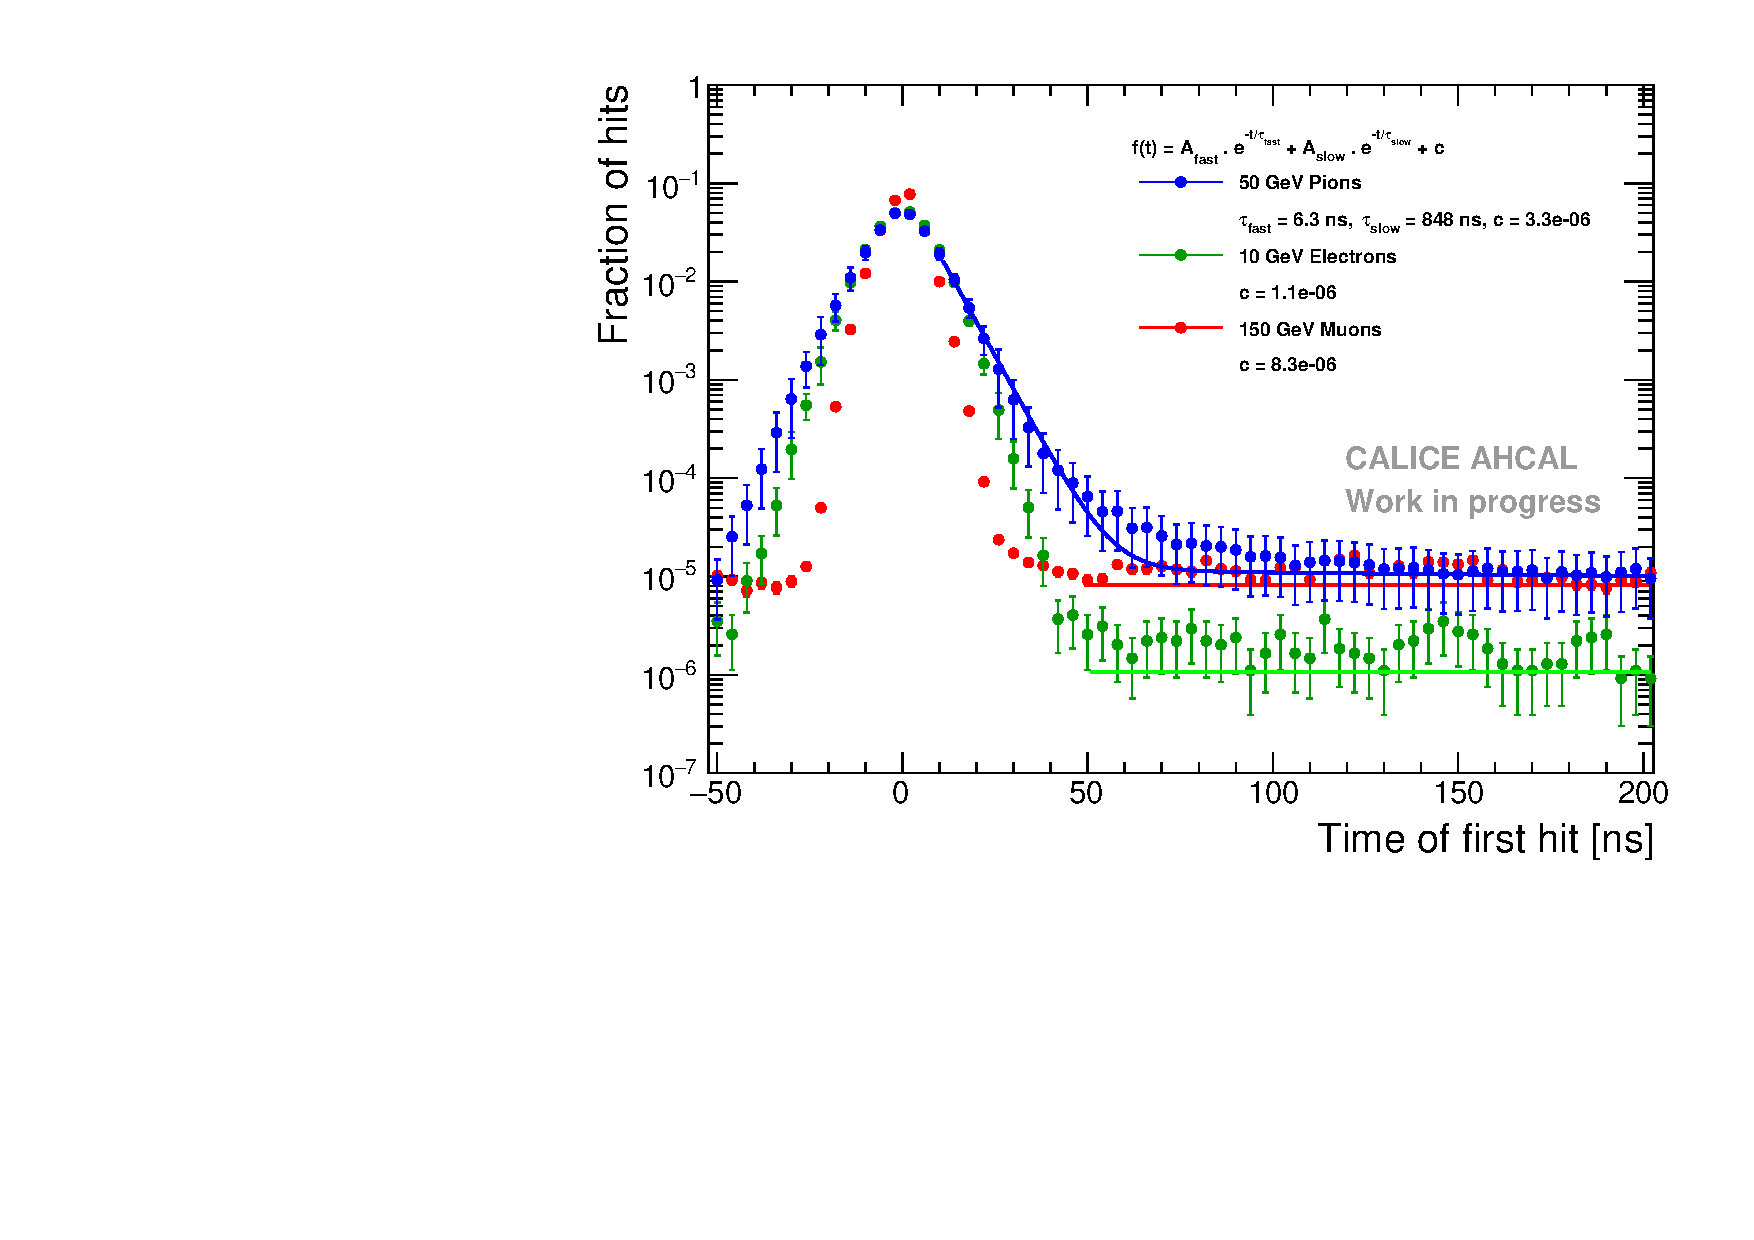
\includegraphics[width=0.6\textwidth]{../Thesis_Plots/Timing/Pions/Plots/Timing_dNdt_Comparison.pdf}
	\caption{Time of first hit for muons, electrons and pions in steel absorber in a range of -50 to 200 ns. The histograms are normalized to the number of events. The lines represent the fit to the data as explained in the text.}
	\label{fig:dNdt_Comparison}
\end{figure}

The figure \ref{fig:dNdt_Comparison} shows the time of first hit for muons, 10 GeV electrons and 50 GeV pions. Energy depositions from muons and electrons are instantaneous within a certain time window centered around 0 ns that is determined by the intrinsic time resolution of the detector. Some isolated hits are present in the tails most likely caused by SiPM thermal noise. This gives an idea of the noise level as well as the rejection of noise in the analysis. One can remark that the noise level in electron data is lower than in the muon data. The reason is not clear. It may come from the difference in beam rate and differences in the detector threshold configurations for different beams.

For muons, around 2\% of hits are later than 50 ns compared to the core of the distribution between -50 and 50 ns. For electrons, 0.37\% of hits are later than 50 ns. For pions, about 1.5\% of hits are after 50 ns. Moreover, the pion time distribution presents a higher tail between 30 to 50 ns than in the electron time distribution. In order to characterize the distribution, a model of the sum of two exponentials and a constant, similar as the T3B experiment \cite{Simon2013} is applied following the equation \ref{eq:dNdt_eq}:

\begin{equation} \label{eq:dNdt_eq}
	\frac{1}{N}\frac{dN}{dt} = A_{fast} \times e^{-\frac{t}{\tau_{fast}}} + A_{slow} \times e^{-\frac{t}{\tau_{slow}}} + c
\end{equation}

where $A_{fast}, \tau_{fast}$ and $A_{slow}, \tau_{slow}$ are the amplitudes and decays times of the modeled fast and slow component of the hadronic shower. Since the fit is performed on several orders of magnitudes, the same fitting method that the T3B experiment uses is applied. It is done in two steps. First, the slow component is fitted between 90 ns and \SI{2}{\micro\second}. Then, fixing the parameters of the slow component, the fast component is fitted between 10 ns to \SI{2}{\micro\second}.

With this procedure, a fast component of $7.04 \pm 0.59$ ns and a slow component of $826 \pm 183$ ns are fitted. The time constant of the fast component is in the same order of magnitude as given by T3B of 8 ns and is interpreted by the evaporation neutrons energy depositions in the active medium. But due to the time resolution of the AHCAL being in the same order of magnitude, it is difficult to confirm this origin.

On the other hand, the time constant of the slow component is very different than in the T3B experiment (around 80 ns in steel). This may be due to the contribution of SiPM noise which reduces the sensitivity to this slow component in the shower. One can remark that this model may be incomplete as the fitting function does match well the data in the transition region of 50 to 100 ns. This is similarly observed in the T3B data. The table \ref{table:dNdt_fit} sums up the fitted results.

\begin{table}[htb!]
	\centering
	\caption{Summary of the fit results in figure \ref{fig:dNdt_Comparison}.}
	\label{table:dNdt_fit}
	\begin{tabular}{@{} lccc @{}}
		\toprule
		Parameter & Muon & Electron & Pion \\
		\midrule
		$\tau_{fast}$ [ns] & - & - & $7.04 \pm 0.59$ \\
		$\tau_{slow}$ [ns] & - & - & $826 \pm 183$ \\
		$c$ & $(7.91 \pm 0.09) \times 10^{-6}$ & $(1.20 \pm 0.02) \times 10^{-6}$ & $(3.38 \pm 0.56) \times 10^{-6}$ \\
		\bottomrule
	\end{tabular}
\end{table}

The figure \ref{fig:dNdt_SimData_10GeV} shows the time distribution of first hits compared with three different physics lists for 10 GeV pions. Additional distribution for higher pion beam energies are shown in appendix \ref{appendix:TimingAdd}. For the core of the distribution under 50 ns, generally, all physics lists describe relatively well the data within systematics. From 10 to 50 GeV, QGSP\_BERT\_HP reproduces well the distribution. Above 50 GeV, the late tail is well described in the simulation but between 50 and 100 ns, it is not well reproduced and under-estimated. QBBC tends to over-estimate the late tail by around a factor 2. This does not agree with the observations made in the T3B experiment were QBBC agreed well with the time distribution for pions of 60 GeV. It may be related to the use of different \geant versions as T3B used \geant v9.4p03. For all distributions, QGSP\_BERT over-estimates the tail of the distribution by around a factor 10.

\begin{figure}[htbp!]
	\centering
	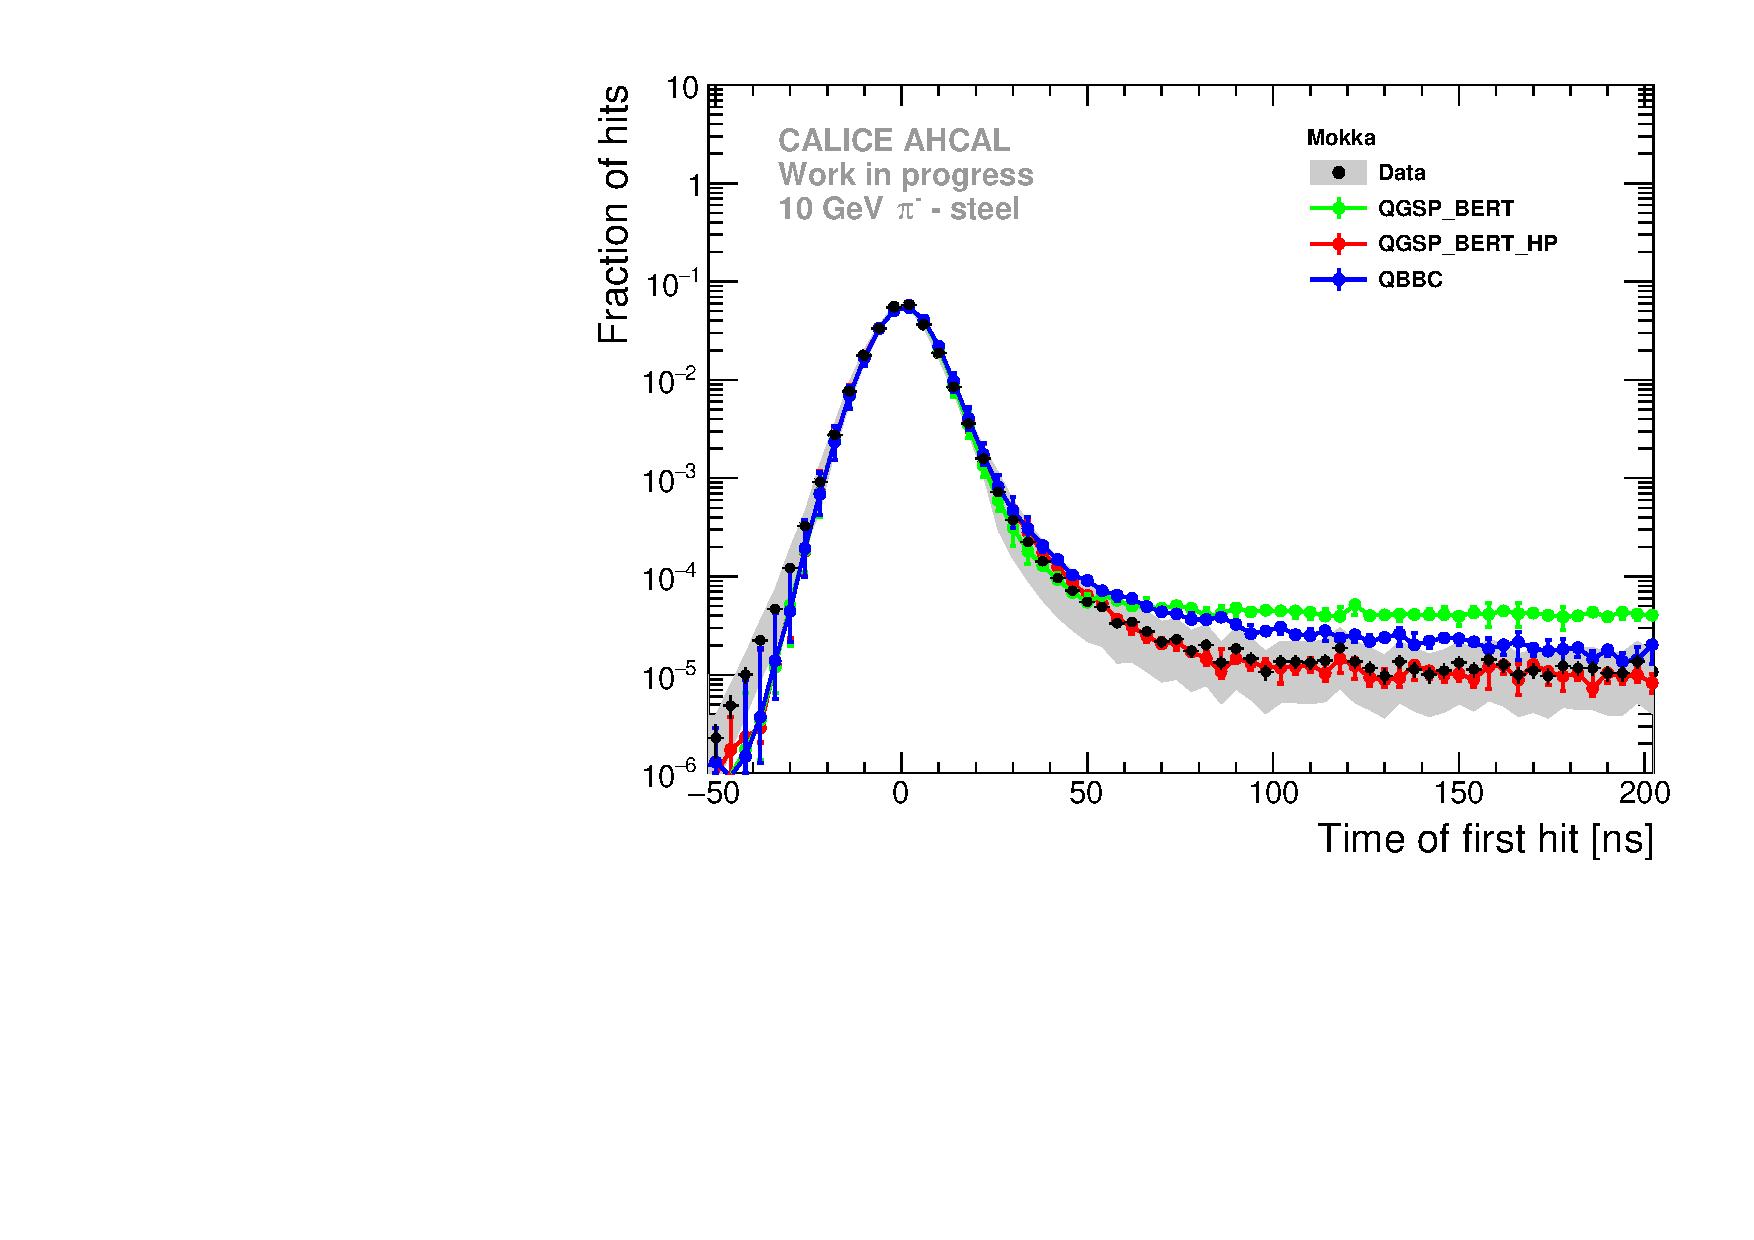
\includegraphics[width=0.6\textwidth]{../Thesis_Plots/Timing/Pions/Plots/Comparison_SimData_Pion10GeV_LateClusters.pdf}
	\caption{Comparison of the time of first hit per bin time for 10 GeV pions in data and six different simulations. The grey and color bands shows the statistical and systematic uncertainties.}
	\label{fig:dNdt_SimData_10GeV}
\end{figure}

\subsection{Energy dependence of the time of first hit}

The energy dependence of the timing of hits has been studied as shown in figure \ref{fig:Energy_Comparison}. the figure shows the mean time of first hit, taken in a time window between -50 ns and 200 ns, as function of the hit energy for muon, electron and pion beams. For muons and electrons, no dependence on energy is observed as expected as all hits are prompt. For pions, a delay of 2-3 ns at 0.5 MIP is observed and decreases down to 0-1 ns above 1 MIP. For higher pion energies than 10 GeV, a decrease in the mean time of the first hit can be observed between 0.5 and 1.5 MIP. Individual distributions have been checked, an example is shown in figure \ref{fig:TimeBinsEnergy} for 90 GeV pions. After 1.5 MIP, the time distribution gets wider and the maximum of the distribution is de-centered slightly from 0 ns, therefore explaining the increase of the mean time of the first hit for hit energies over 1.5 MIP.

\begin{figure}[htbp!]
	\begin{subfigure}[t]{0.5\textwidth}
		\centering
		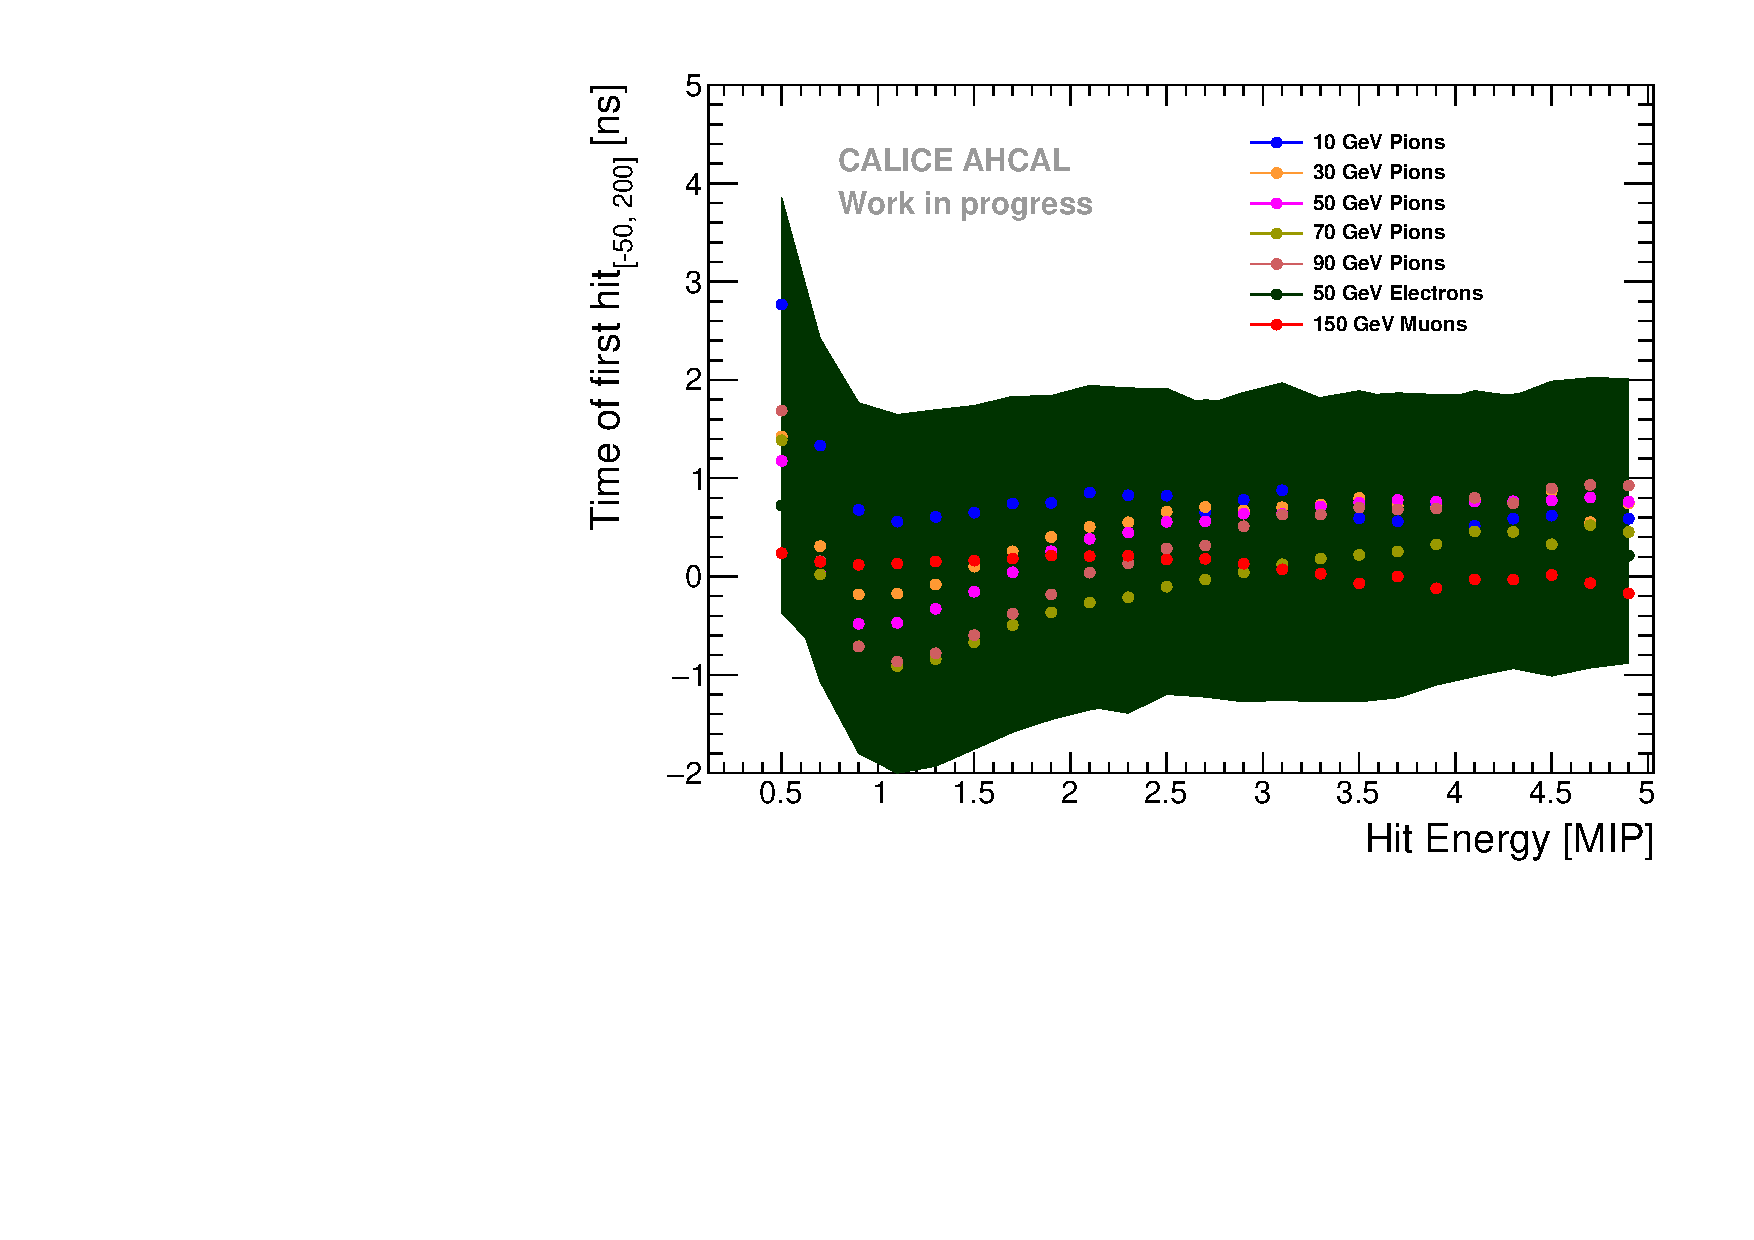
\includegraphics[width=1\textwidth]{../Thesis_Plots/Timing/Pions/Plots/Timing_Energy_Comparison_ShortAsymRange.pdf}
		\caption{} \label{fig:Energy_Comparison}
	\end{subfigure}
	\hfill
	\begin{subfigure}[t]{0.5\textwidth}
		\centering
		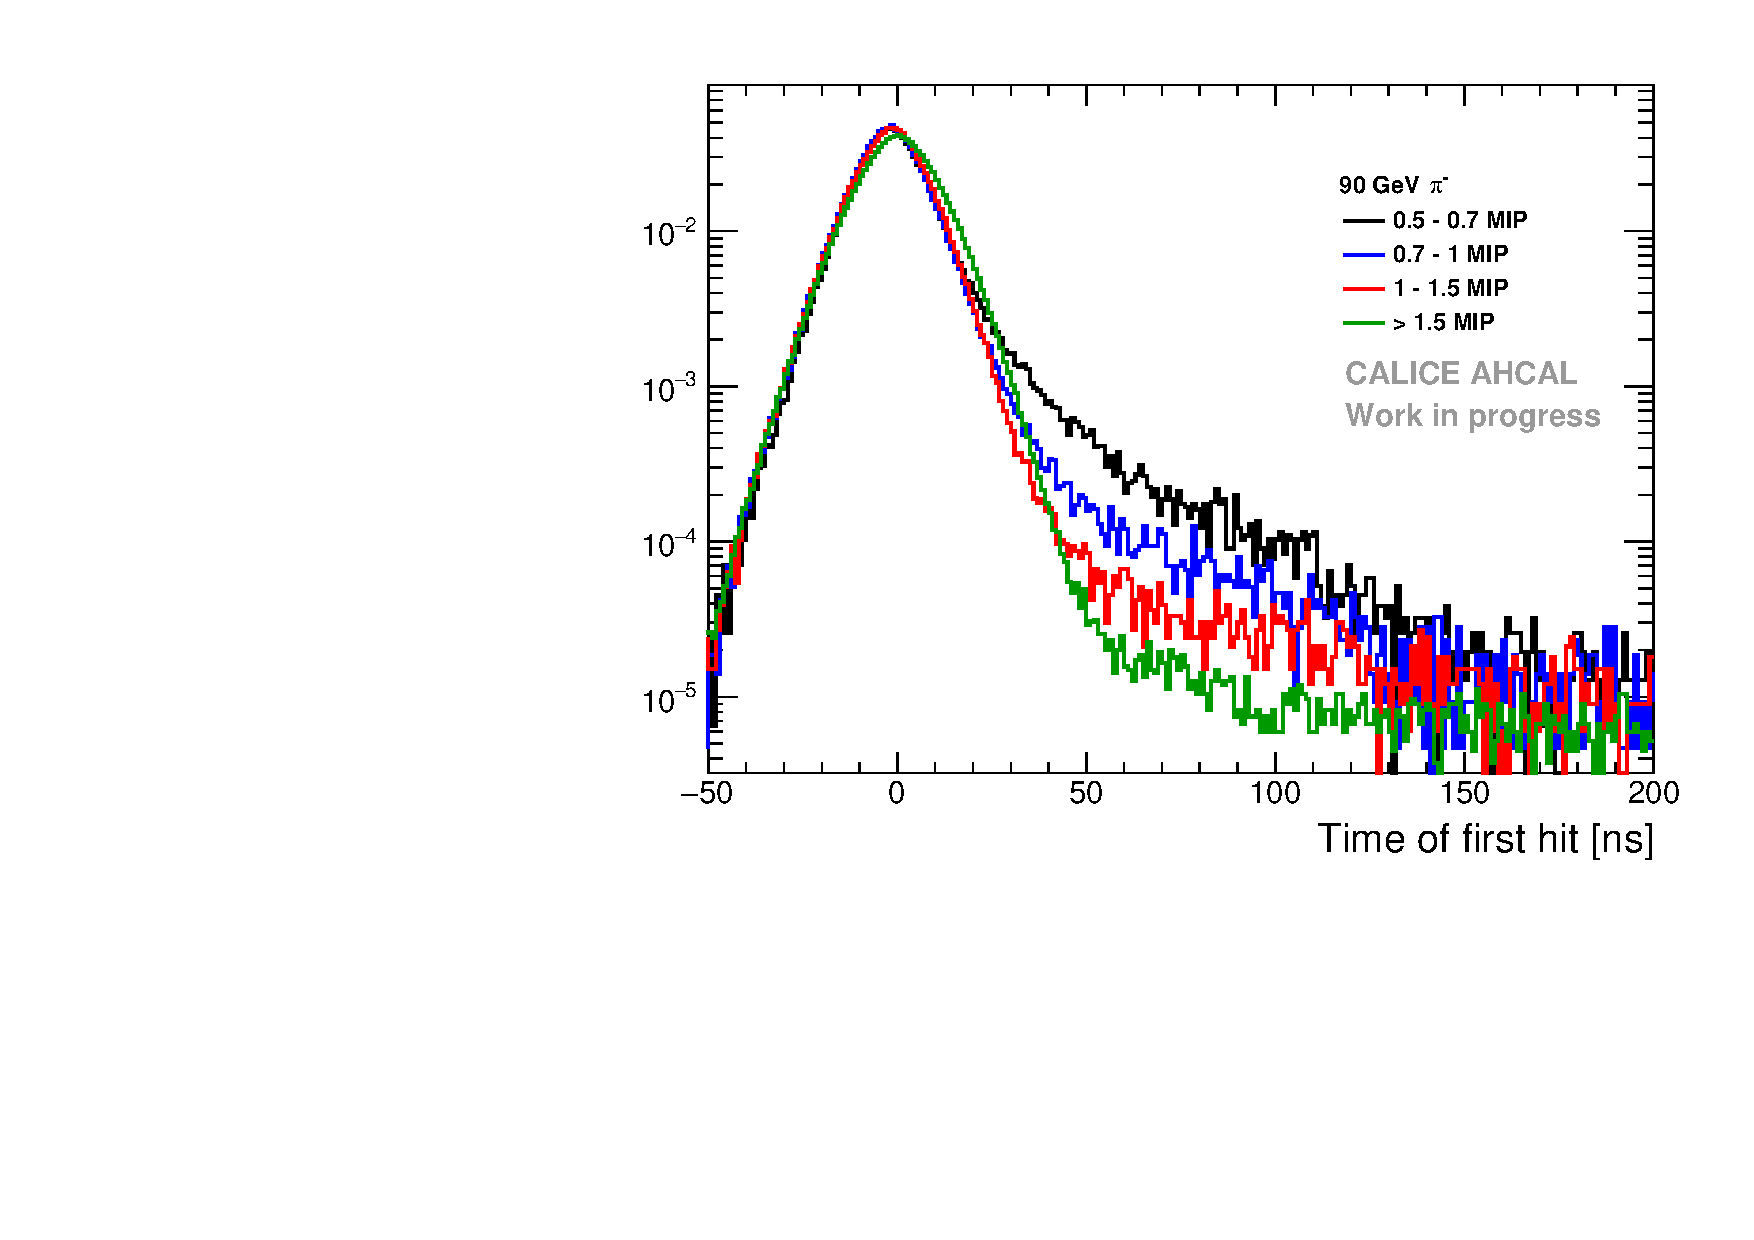
\includegraphics[width=1\textwidth]{../Thesis_Plots/Timing/Pions/Plots/TimeEnergyBinsPions.pdf}
		\caption{} \label{fig:TimeBinsEnergy}
	\end{subfigure}
	\caption{On the left, time of first hit as function of the hit energy for muons, electrons and pions in steel absorber in a range of -50 to 200 ns. The bands represent the systematic uncertainty. On the right, time distribution for 90 GeV pions for different hit energy ranges.}
\end{figure}

The figure \ref{fig:Energy_SimData_10GeV} shows comparison of the mean time of first hit as a function of the hit energy in data and simulations for 10 GeV pions. For higher pion energies, the figures are in appendix \ref{appendix:TimingAdd}. For 10 GeV pions, the simulation reproduces well the data within the systematics. For higher energies, a difference is visible in the region 0.5 to 1.5 MIP where the simulation is above the data. Above around 3 MIPs, the data and simulations agree well. Firstly, a difference is visible between QGSP\_BERT and QGSP\_BERT\_HP mainly between hit energies of 1-3 MIPs but, in general, the difference is smaller than the systematic uncertainty on the data. Secondly, QGSP\_BERT and QBBC are very similar over the full hit energy range. Finally, all models show an increase of the mean time of first hit at small hit energies with higher beam energy. The data does not reflect this.

\begin{figure}[htbp!]
	\centering
	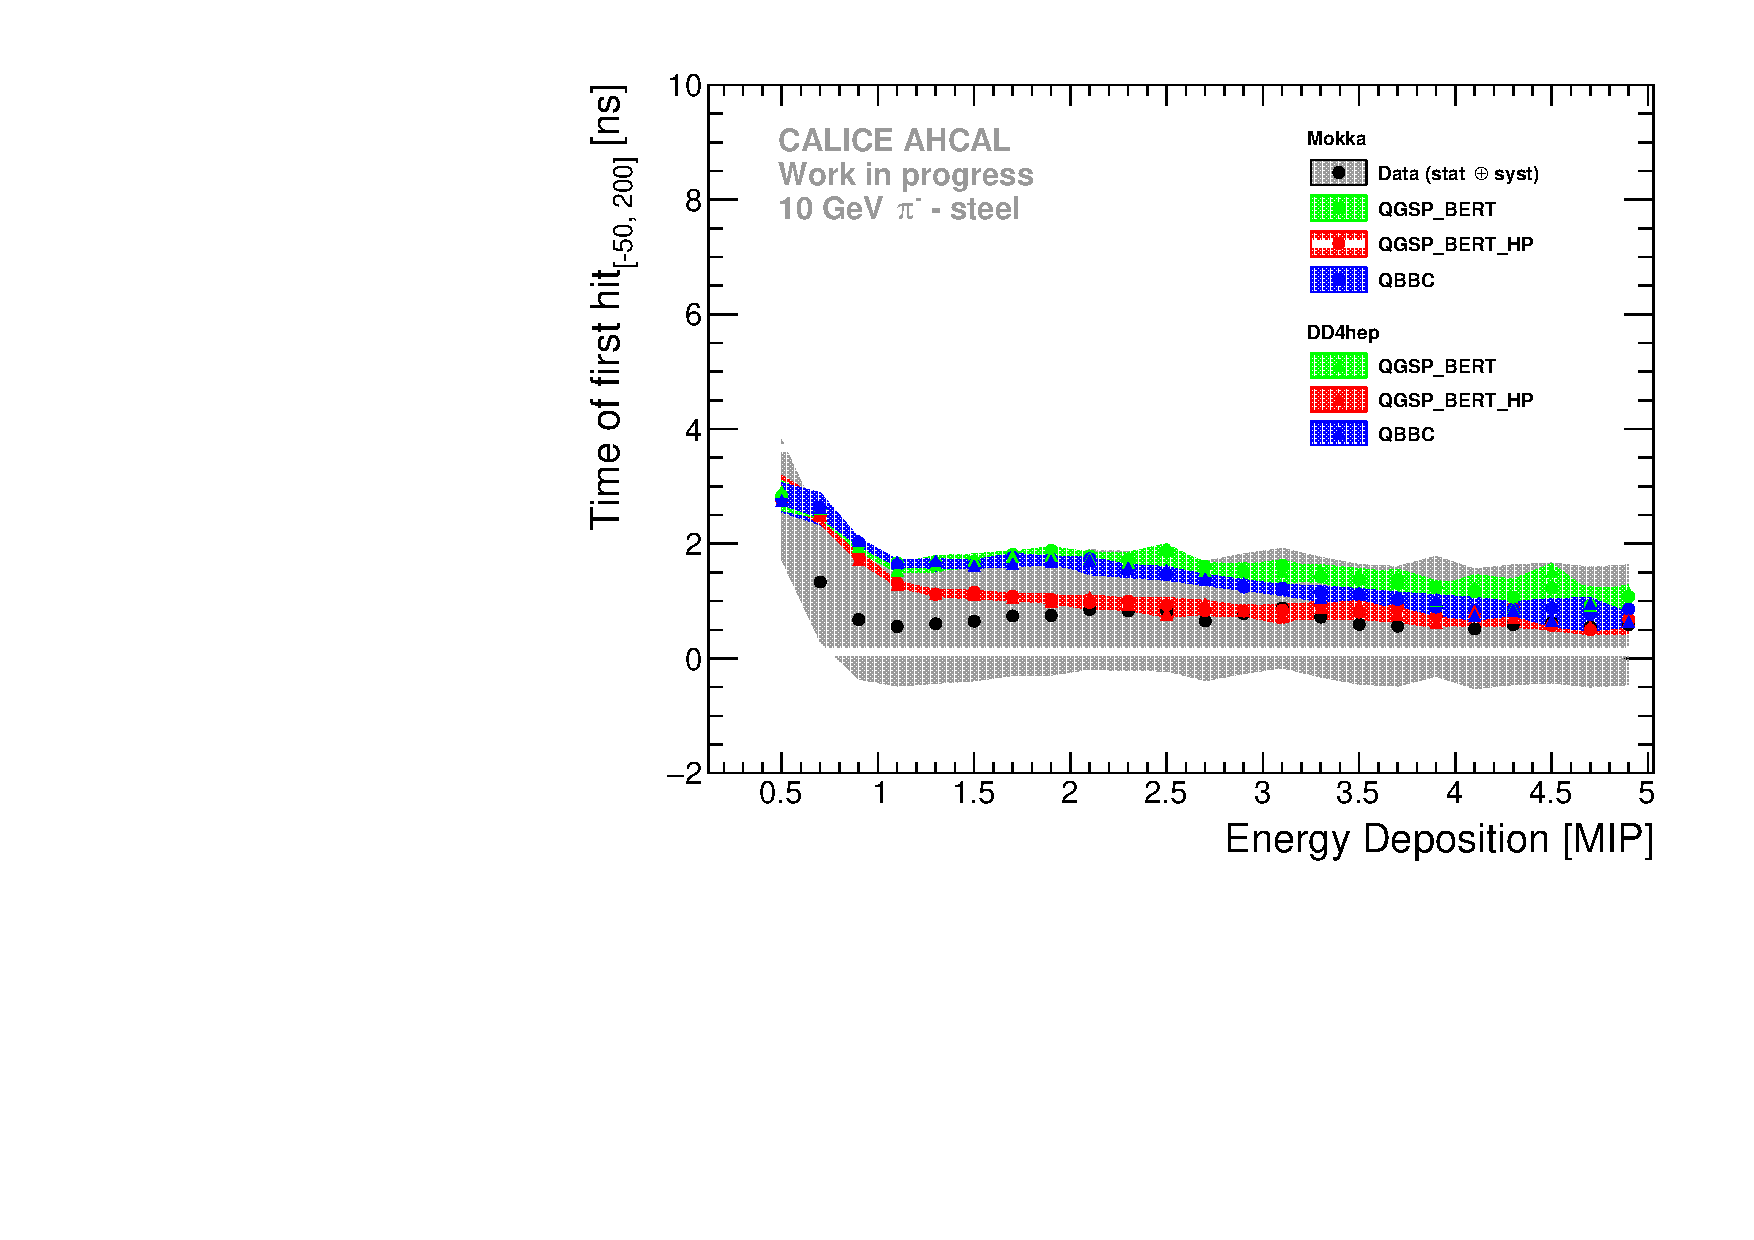
\includegraphics[width=0.6\textwidth]{../Thesis_Plots/Timing/Pions/Plots/ComparisonToSim/Time_Energy_10GeV.pdf}
	\caption{Comparison of the mean time of first hit as function of the hit energy in data and simulations for 10 GeV pions. The grey and color bands shows the statistical and systematic uncertainties.}
	\label{fig:Energy_SimData_10GeV}
\end{figure}

This comparison seems to confirm that low energy hits are responsible for delayed energy depositions in the calorimeter. This is most likely due to low energy neutrons from capture and spallation processes. Higher energy deposits occur mostly in the prompt part of the hadron shower.

\subsection{Radial dependence of the time}

The prompt component of a hadron shower is dominated by EM sub-showers and relativistic particles, whereas the delayed component is coming from mostly evaporation and spallation low energy neutrons. It is expected that the former is concentrated near the shower axis, while the latter, is spread out laterally as these neutrons can travel far away in the calorimeter before interacting.

This is investigated by looking at the mean time of first hit as a function of the hit distance to the shower center of gravity defined in the [x,y] plane. For the muon data, the hit position in the detector relative to (0,0) is used. This is shown in figure \ref{fig:Radius_Comparison_SSF} for the layers 3 to 10 and in figure \ref{fig:Radius_Comparison_BL} the layers 11 to 14 separately. The layers were separated due to a decrease of the mean time of first hit
at the radius transition of a small layer (3 to 10) and a big layer (11 to 14). This is thought to be related to the fact that the radius dependence may depend on the starting point of the pion shower. This is investigated in more details in section \ref{sec:TimeRadiusDepth}.

\begin{figure}[htbp!]
	\begin{subfigure}[t]{0.5\textwidth}
		\centering
		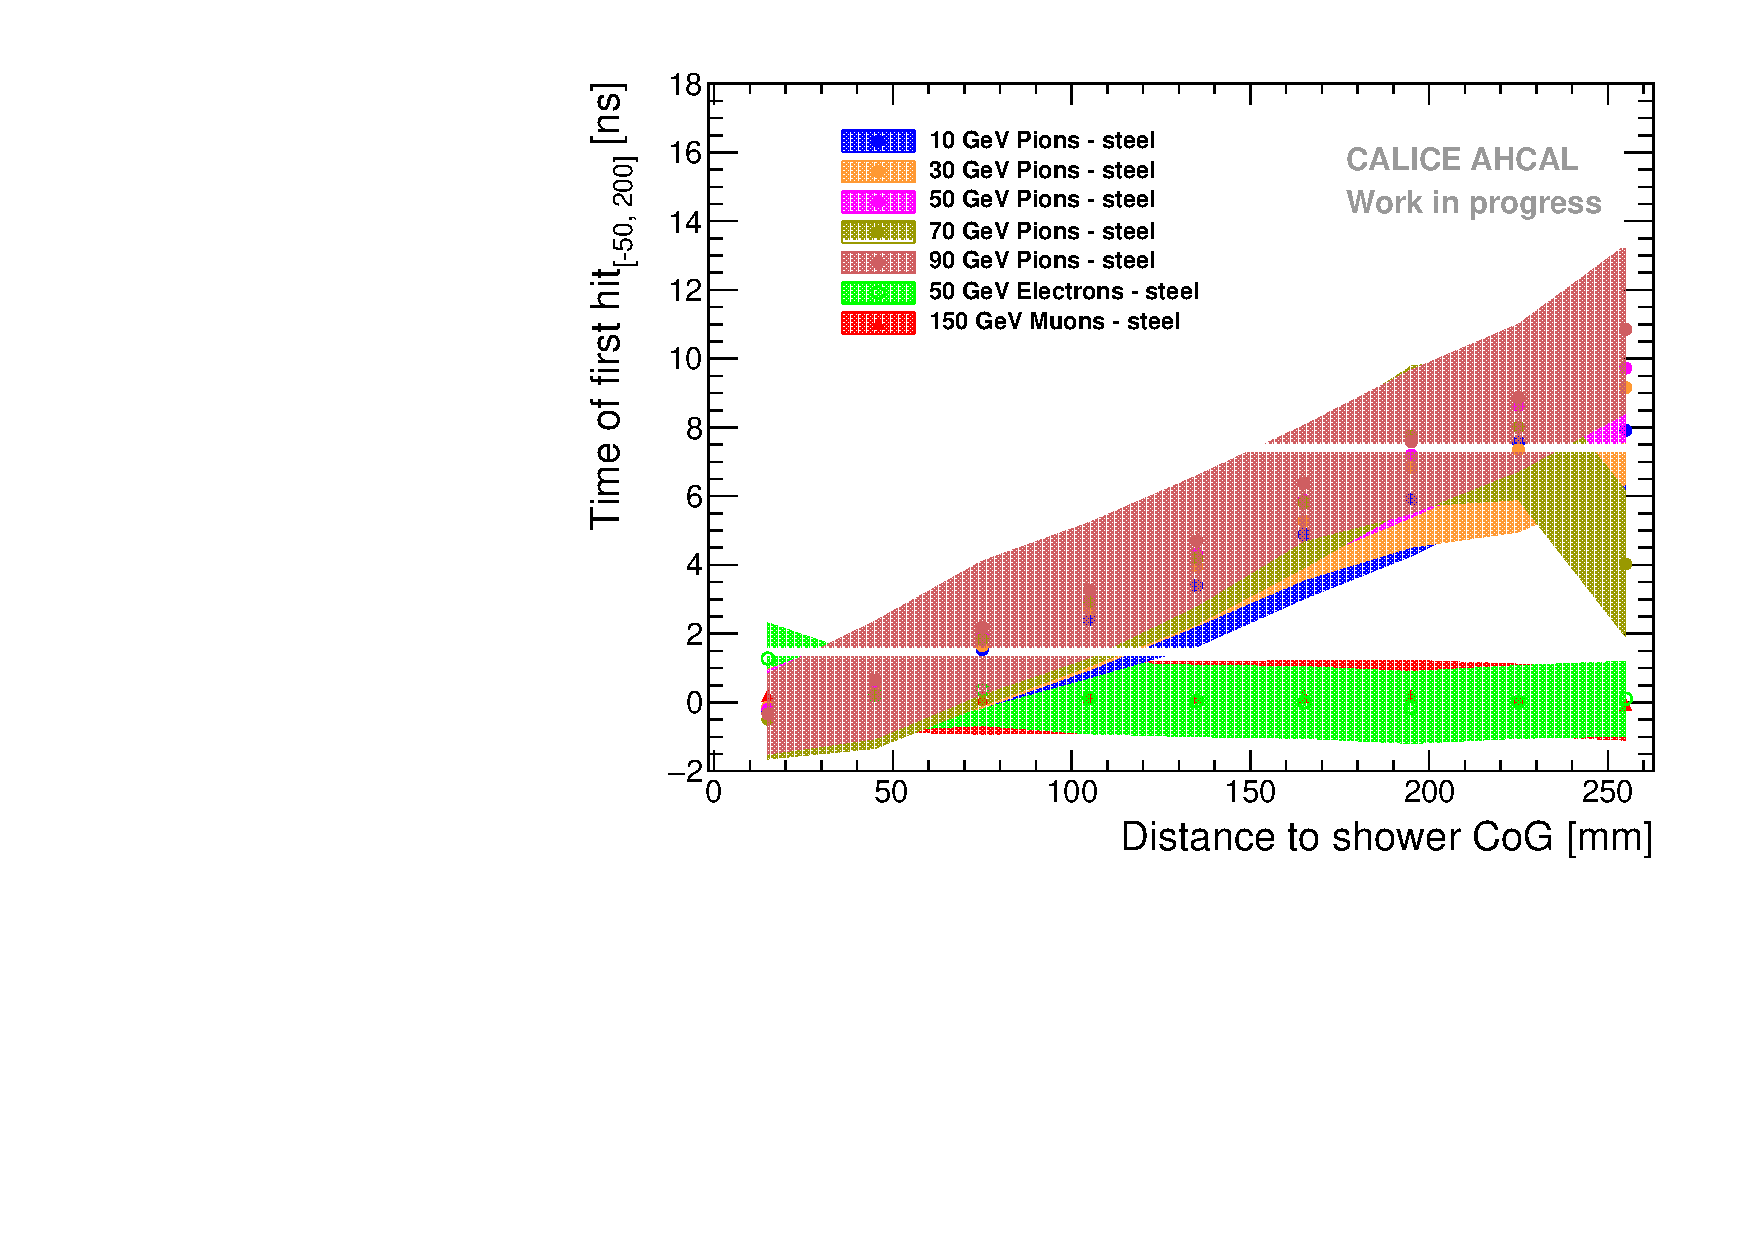
\includegraphics[width=1\textwidth]{../Thesis_Plots/Timing/Pions/Plots/Timing_Radius_Comparison_ShortAsymRange_SSF.pdf}
		\caption{Layers 3 to 10.}\label{fig:Radius_Comparison_SSF}
	\end{subfigure}
	\hfill
	\begin{subfigure}[t]{0.5\textwidth}
		\centering
		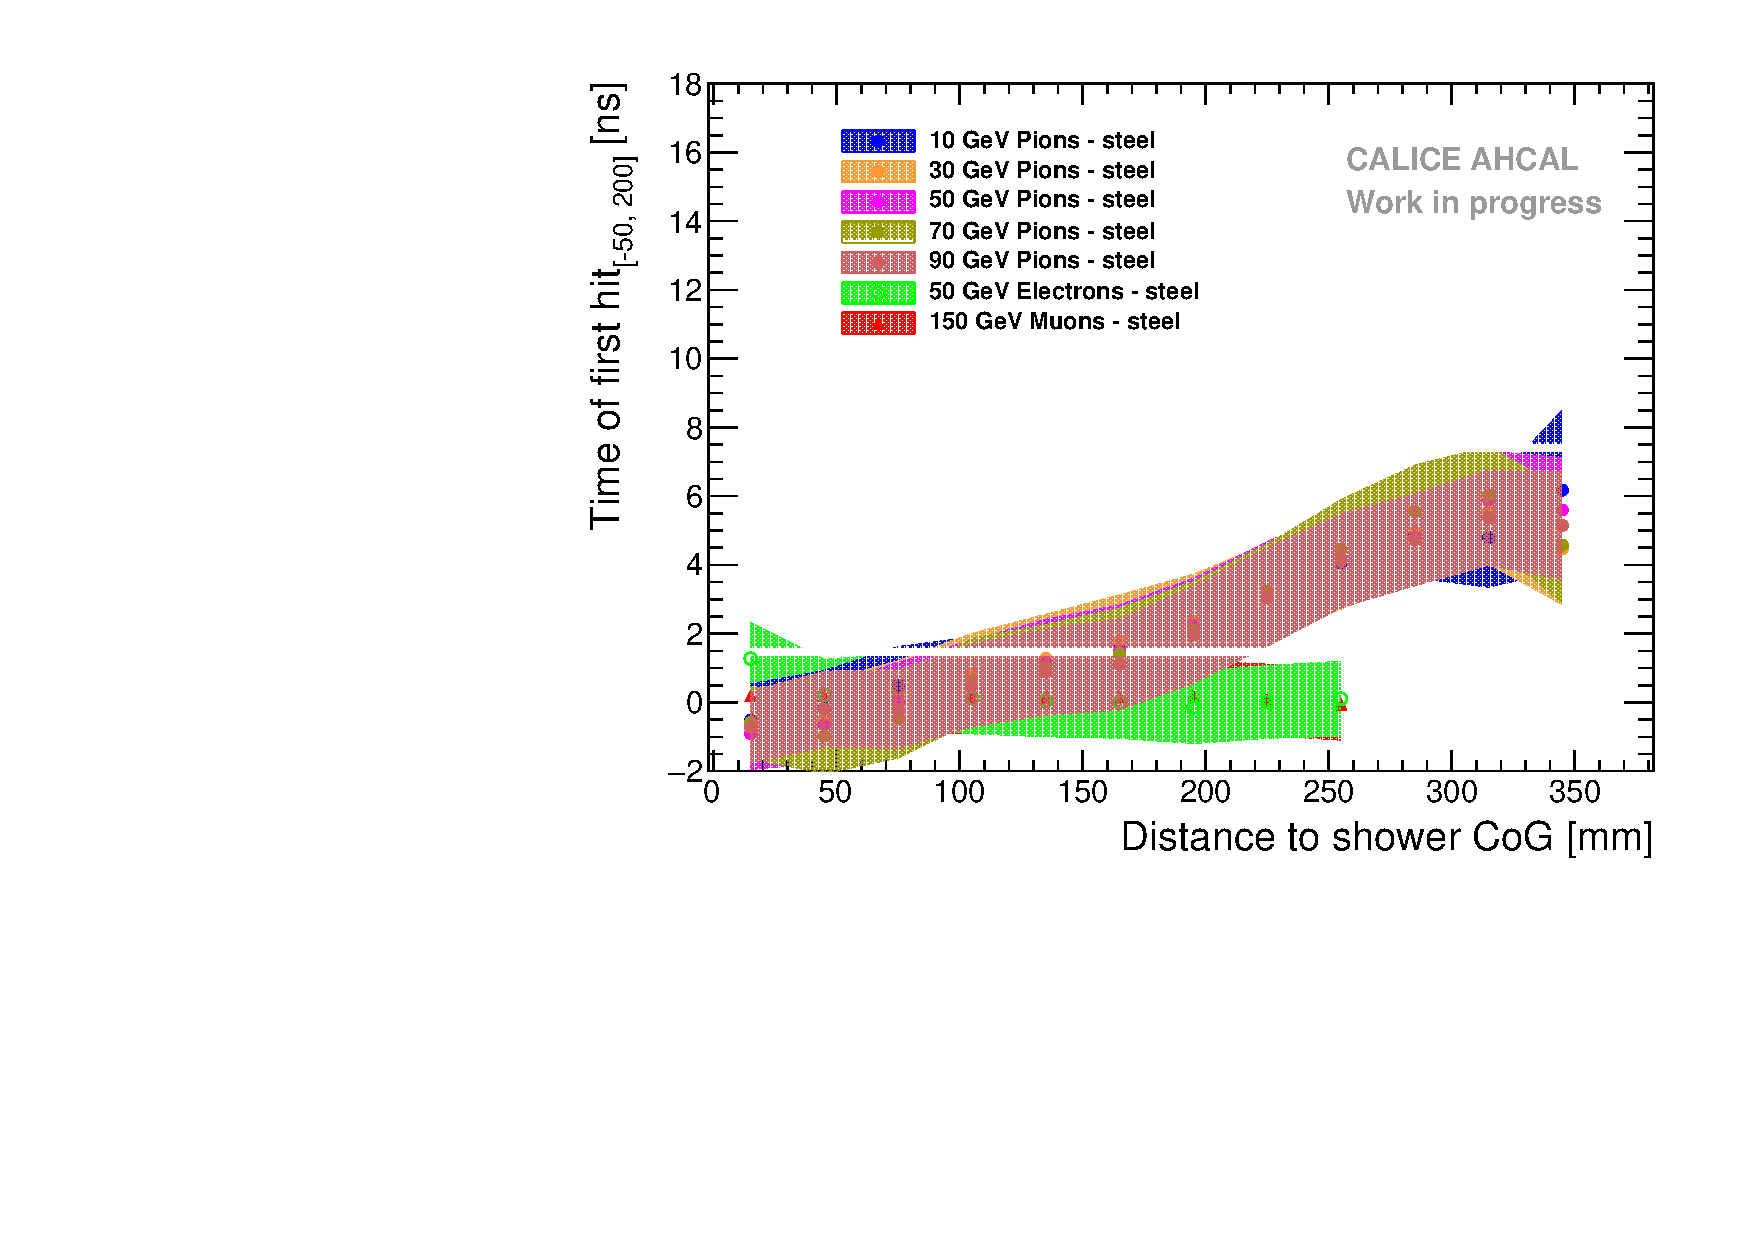
\includegraphics[width=1\textwidth]{../Thesis_Plots/Timing/Pions/Plots/Timing_Radius_Comparison_ShortAsymRange_BL.pdf}
		\caption{Layers 11 to 14.}\label{fig:Radius_Comparison_BL}
	\end{subfigure}
	\caption{Radial shower timing profile of the time of first hit for muon, electron and pion beams. The left plot shows the timing profile for the small layers and the right profile shows the timing profile for big layers. The explanation for the separation is described in the text. The systematics are shown by the color bands.}
	\label{fig:RadialTiming}
\end{figure}

For muons and electrons, the mean time of the first hit does not vary with the increase of radius showing that the processes involved are prompt and independent of the position. On the contrary for hadronic showers, it shows an increase of the mean time of the first hit as function of the hit distance to the shower axis. As well, there is no dependence on the energy of the shower. However, the layers 3 to 10 present a steeper slope by around 50\% than for the layers 11 to 14 (from $\sim$1 ns per tile to $\sim$0.5 ns per tile).

Nevertheless, the observation is consistent with the expectation of the core of the shower depositing promptly most of the energy via EM sub-showers and relativistic particles near the shower axis. This is followed by a hadronic halo which contributes to delayed signals by mainly neutron-induced processes. For the layers 3 to 10, the mean time of first hit varies between 0 ns at small radius and 10 ns at 25 cm. For the layers 11 to 14, it varies between 0 ns near the shower axis, 4 ns at 25 cm and 6 ns at 35 cm.

\begin{figure}[htbp!]
	\begin{subfigure}[t]{0.5\textwidth}
		\centering
		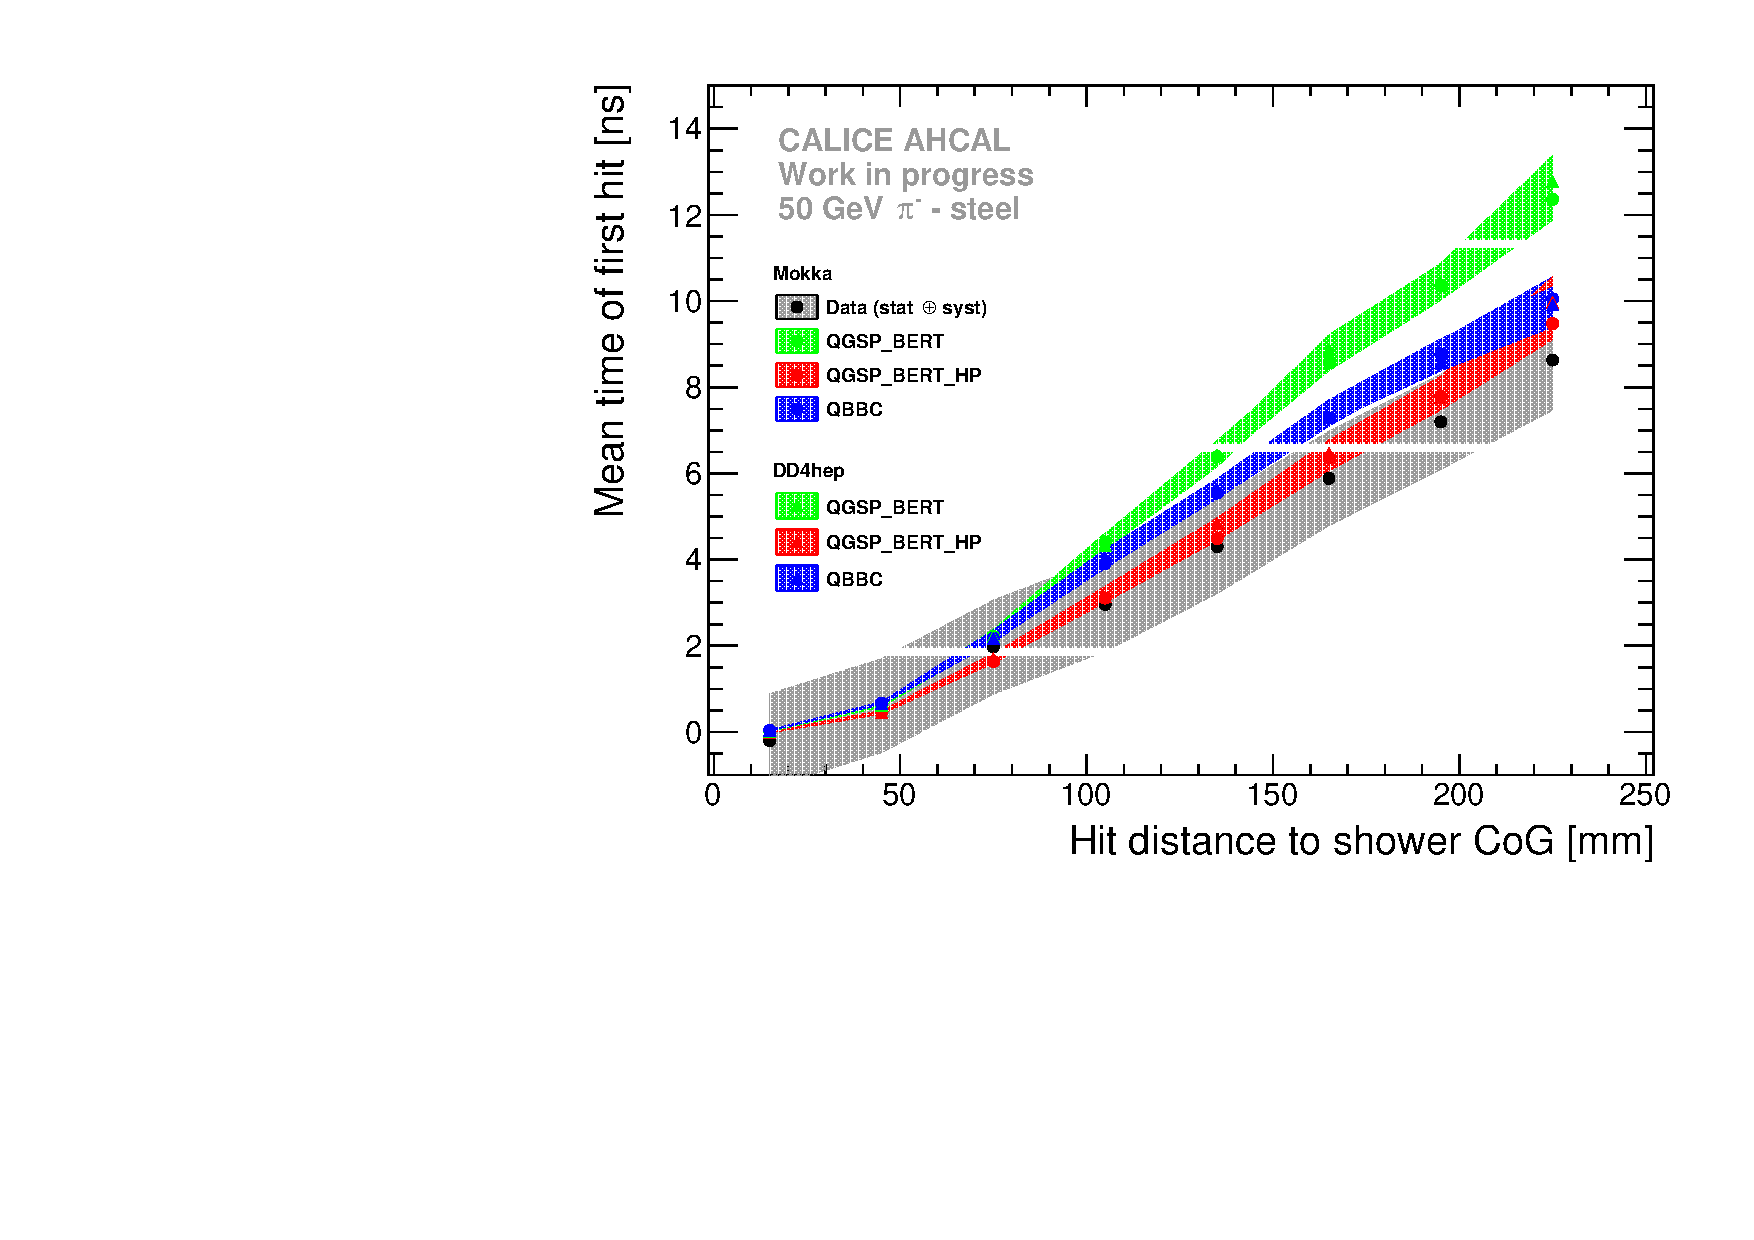
\includegraphics[width=1\textwidth]{../Thesis_Plots/Timing/Pions/Plots/ComparisonToSim/Time_Radius_50GeV_SSF.pdf}
		\caption{} \label{fig:Radius_SSF_SimData_50GeV}
	\end{subfigure}
	\hfill
	\begin{subfigure}[t]{0.5\textwidth}
		\centering
		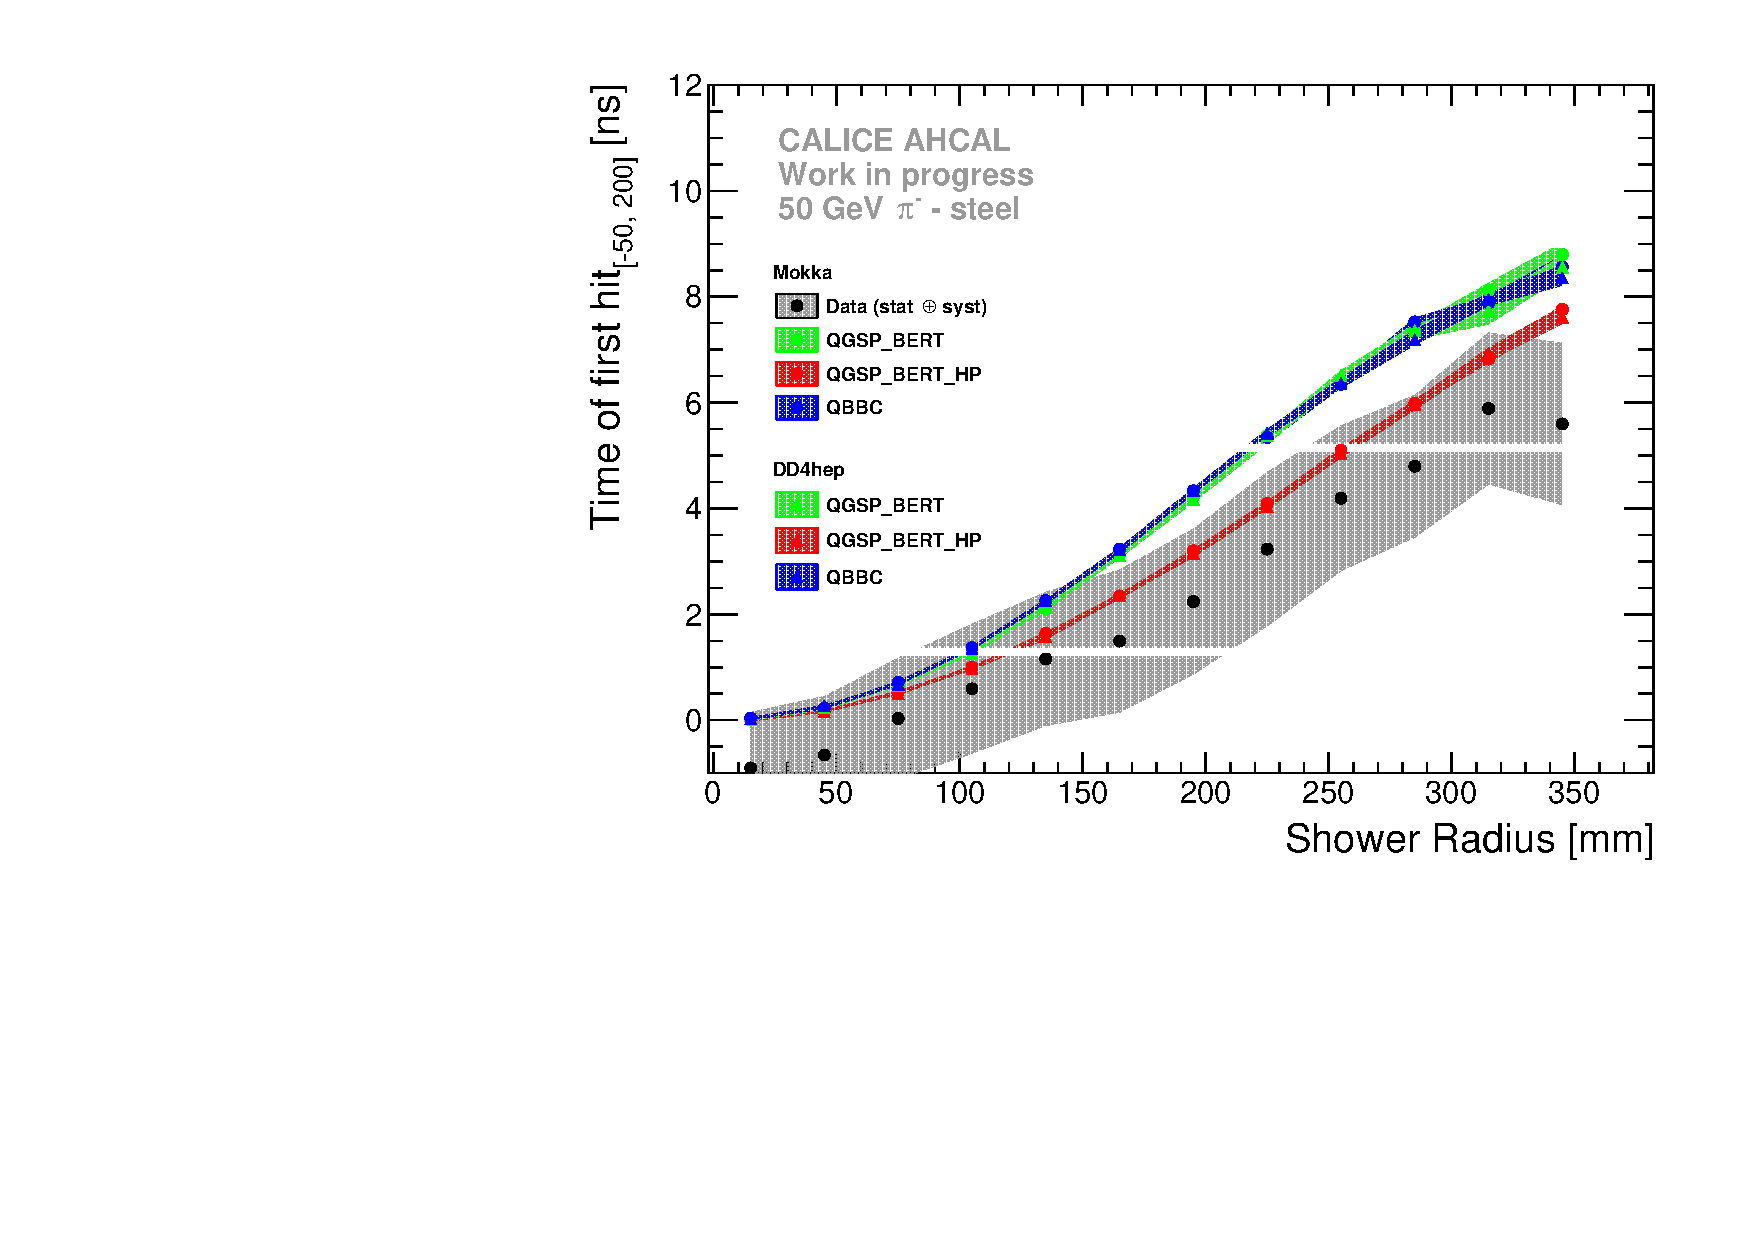
\includegraphics[width=1\textwidth]{../Thesis_Plots/Timing/Pions/Plots/ComparisonToSim/Time_Radius_50GeV_BL.pdf}
		\caption{} \label{fig:Radius_BL_SimData_50GeV}
	\end{subfigure}
	\caption{Comparison of the time of first hit as function of the hit distance to the shower axis in data and simulations for 50 GeV pion for the layers 3 to 10 on the left and for layers 11 to 14 on the right. The grey and color bands shows the systematics.}
	\label{fig:Radius_SSF_SimData_50GeVComparison}
\end{figure}

The radial dependence of the time of first hit of 50 GeV pion showers is compared to simulations as shown in figure \ref{fig:Radius_SSF_SimData_50GeVComparison}. For other energies, the figures are in appendix \ref{appendix:TimingAdd}. For the small layers, the physics lists QBBC and QGSP\_BERT\_HP reproduce well the data within systematics. QGSP\_BERT agrees well under 10 cm and starts to deviate up to 4-6 ns at 23 cm. Concerning the big layers, over the full energy range, QGSP\_BERT\_HP physics list agrees the best with the data. QBBC and QGSP\_BERT agree with data up to around 10 cm radius and then lie above the data for the mean time of first hit. The difference with the data varies between few ns to 3-4 ns between 17 cm to 35 cm radius. This confirms that without precision neutron tracking, too many late energy depositions are created that are spread far away from the shower axis.

\subsubsection{Time dependence with the shower depth}
\label{sec:TimeRadiusDepth}

To complement this, a dependence of the mean time of first hit as function of the hit distance to the center of gravity of the shower for different layers, corresponding to different shower depths, is shown in figure \ref{fig:Radius_Indivi}. A dependency of the slope of the curve can be observed as function of the layer. The layer 3 shows a much steeper slope of around 1.8 ns per tile than for the layer 14 at 0.6 ns per tile. This dependency is not fully understood and seems counter intuitive as one would expect more later hits in the last layers. One possibility is that the later component for the first layers could come from the Albedo effect \cite{ELLSWORTH1982167} and backscattered neutrons. It has been studied in simulation also with the QGSP\_BERT\_HP physics list and the same behavior is described by the simulation as shown in figure \ref{fig:Radius_Indivi_Sim}.

\begin{figure}[htbp!]
	\begin{subfigure}[t]{0.5\textwidth}
		\centering
		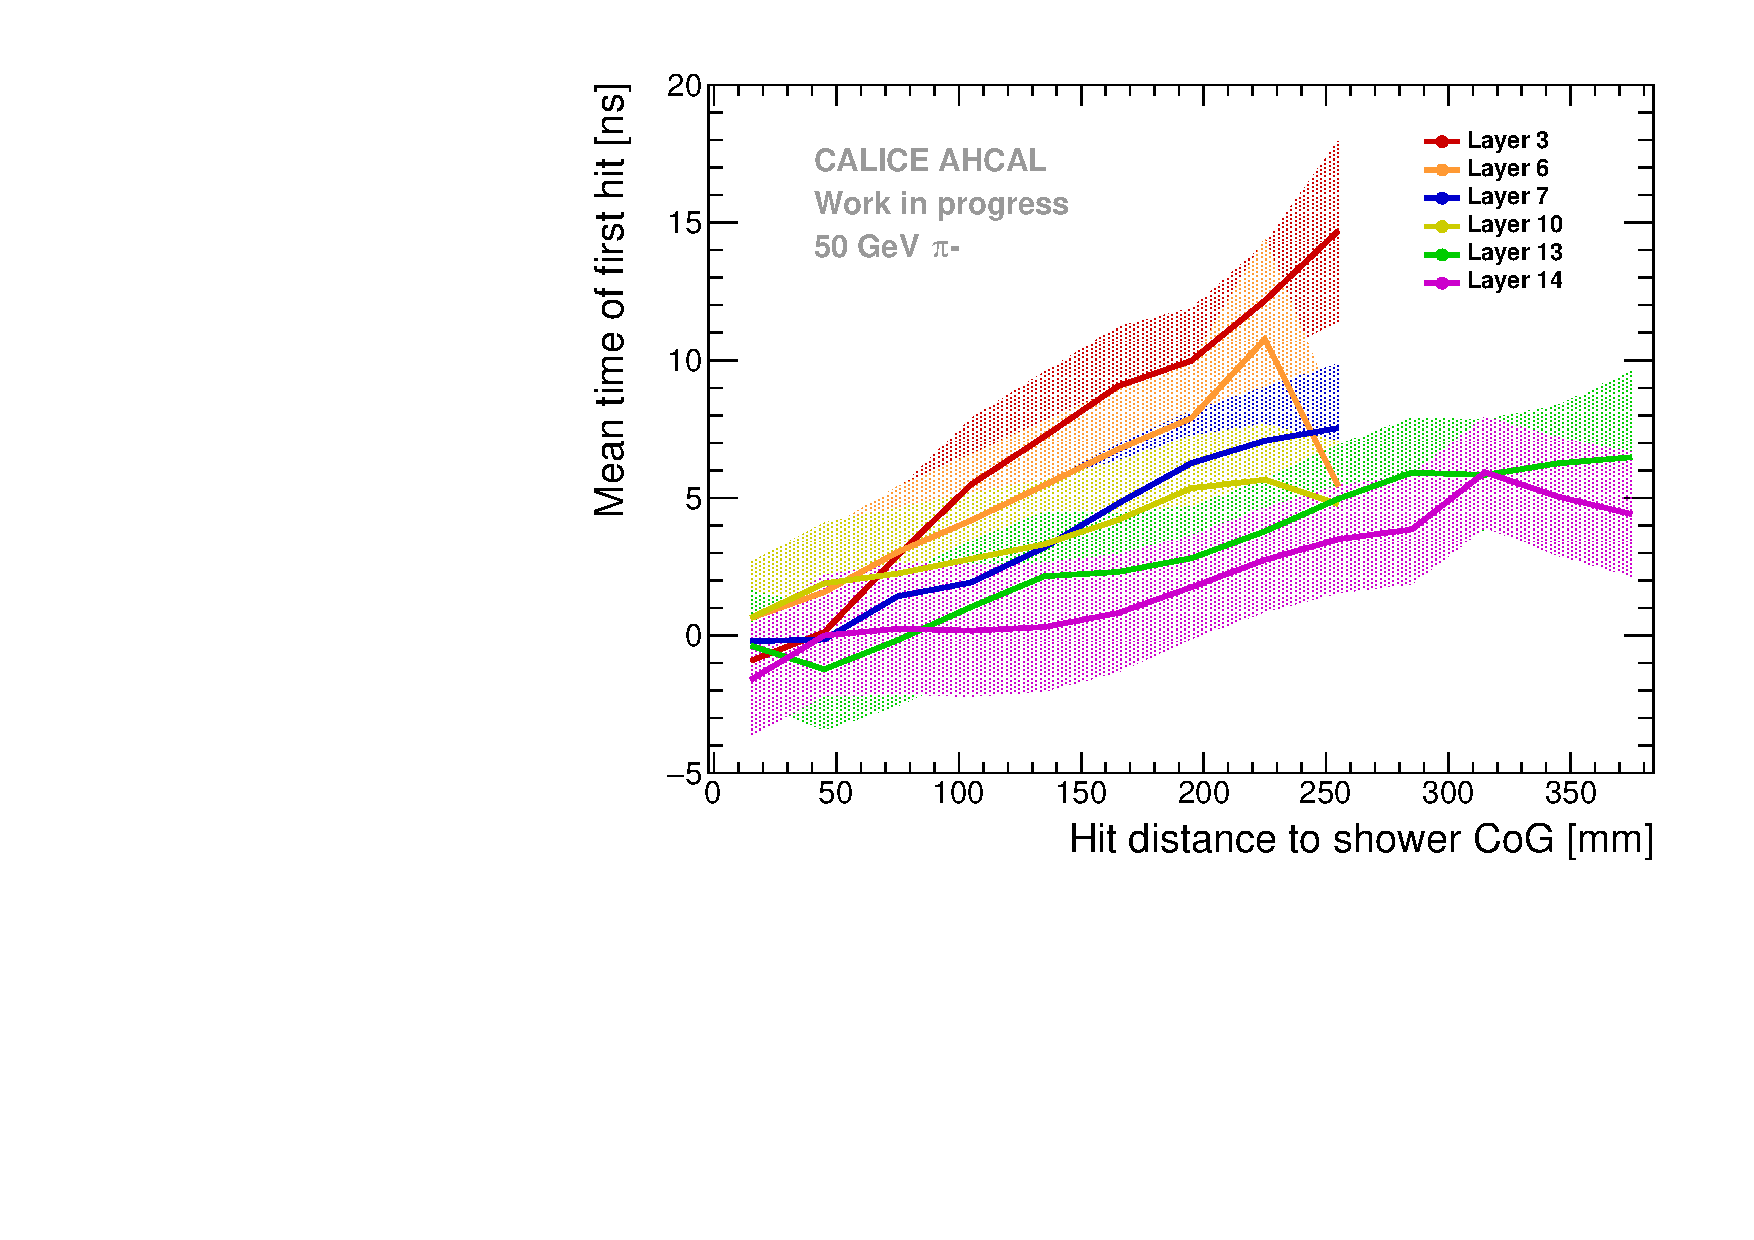
\includegraphics[width=1\textwidth]{../Thesis_Plots/Timing/Pions/Plots/Timing_Radius_Comparison_ShortAsymRange_IndividualLayers.pdf}
		\caption{}\label{fig:Radius_Indivi}
	\end{subfigure}
	\hfill
	\begin{subfigure}[t]{0.5\textwidth}
		\centering
		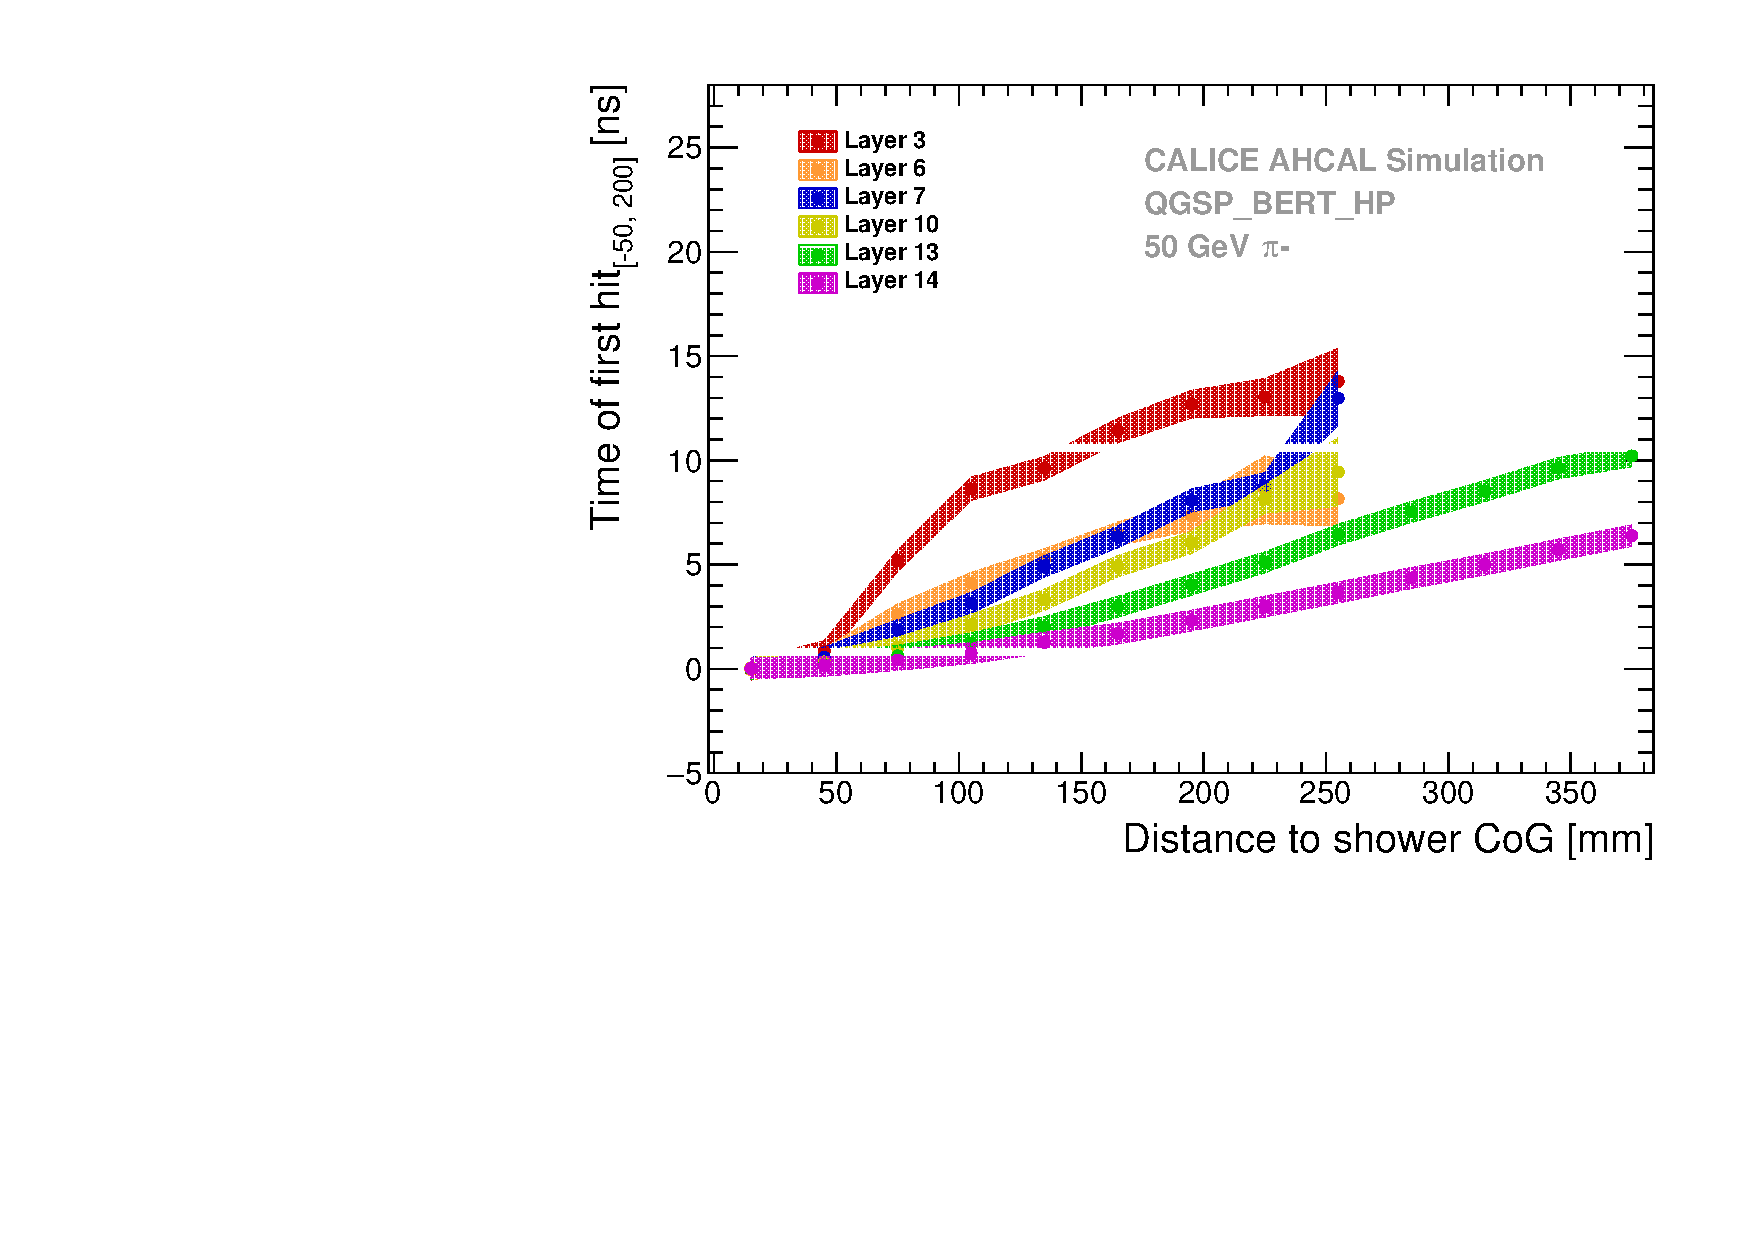
\includegraphics[width=1\textwidth]{../Thesis_Plots/Timing/Pions/Plots/Timing_Radius_Comparison_ShortAsymRange_IndividualLayers_Sim.pdf}
		\caption{}\label{fig:Radius_Indivi_Sim}
	\end{subfigure}
	\caption{Mean time of first hit as function of the hit distance to the center of gravity for 50 GeV pions for different layers. On the left, it is shown for data. On the right, it is shown for simulation using QGSP\_BERT\_HP physics list. Both figures shows the same behavior with a decrease of the curve slope for deeper layers in the calorimeter.}
	\label{fig:Radius_IndiviAll}
\end{figure}

In the following, the mean time of first hit as a function of the hit distance to the shower axis at a constant distance between the layer investigated and the first hard interaction (\acrshort{fhi}) layer of the hadronic shower. The shower start finder algorithm is based on previous work \cite{CaN026} in order find the layer of the first hard interaction. Slight modifications had to be done due to the fact that some of the layers in the front of the detector show a bad performance with many non-working channels.

The basics of the algorithm was to find the primary pion track and to determine the shower start layer. To determine the shower start layer $s_{layer}$, the number of hits $n_{Hits}^{i, i+1}$ in the layer $i$ and $i+1$ is counted. If $n_{Hits}^{i, i+1} > 6$, the shower is considered started between layer $i$ and $i+1$. To determine the correct layer, the energy sum between layer $i$, $i+1$, $i+2$ and $i+3$ is checked such as:
\begin{equation*}
	s_{layer} =
	\begin{cases}
		i, & \text{if} \: E_{sum}^{i+2} < E_{sum}^{i} \:\&\: (E_{sum}^{i+3} < E_{sum}^{i}) \:\&\: (E_{sum}^{i+3} + E_{sum}^{i+2}) < (E_{sum}^{i+1} + E_{sum}^{i}) \\
		i-1, & \text{otherwise}
	\end{cases}
\end{equation*}

Then, if an event was found, a cross-check on the length of the primary track was made. The length of the primary track is required to be over three hits. The performance of the algorithm was evaluated by looking at the difference between the reconstructed layer of the FHI and the Monte-Carlo truth information on the start of the shower. This is shown in figure \ref{fig:FHIAlgo}. The performance of the algorithm is good enough in order to get a good estimate of the FHI layer and has a small tendency to reconstruct the FHI at a deeper layer.

\begin{figure}[htbp!]
	\begin{subfigure}[t]{0.5\textwidth}
		\centering
		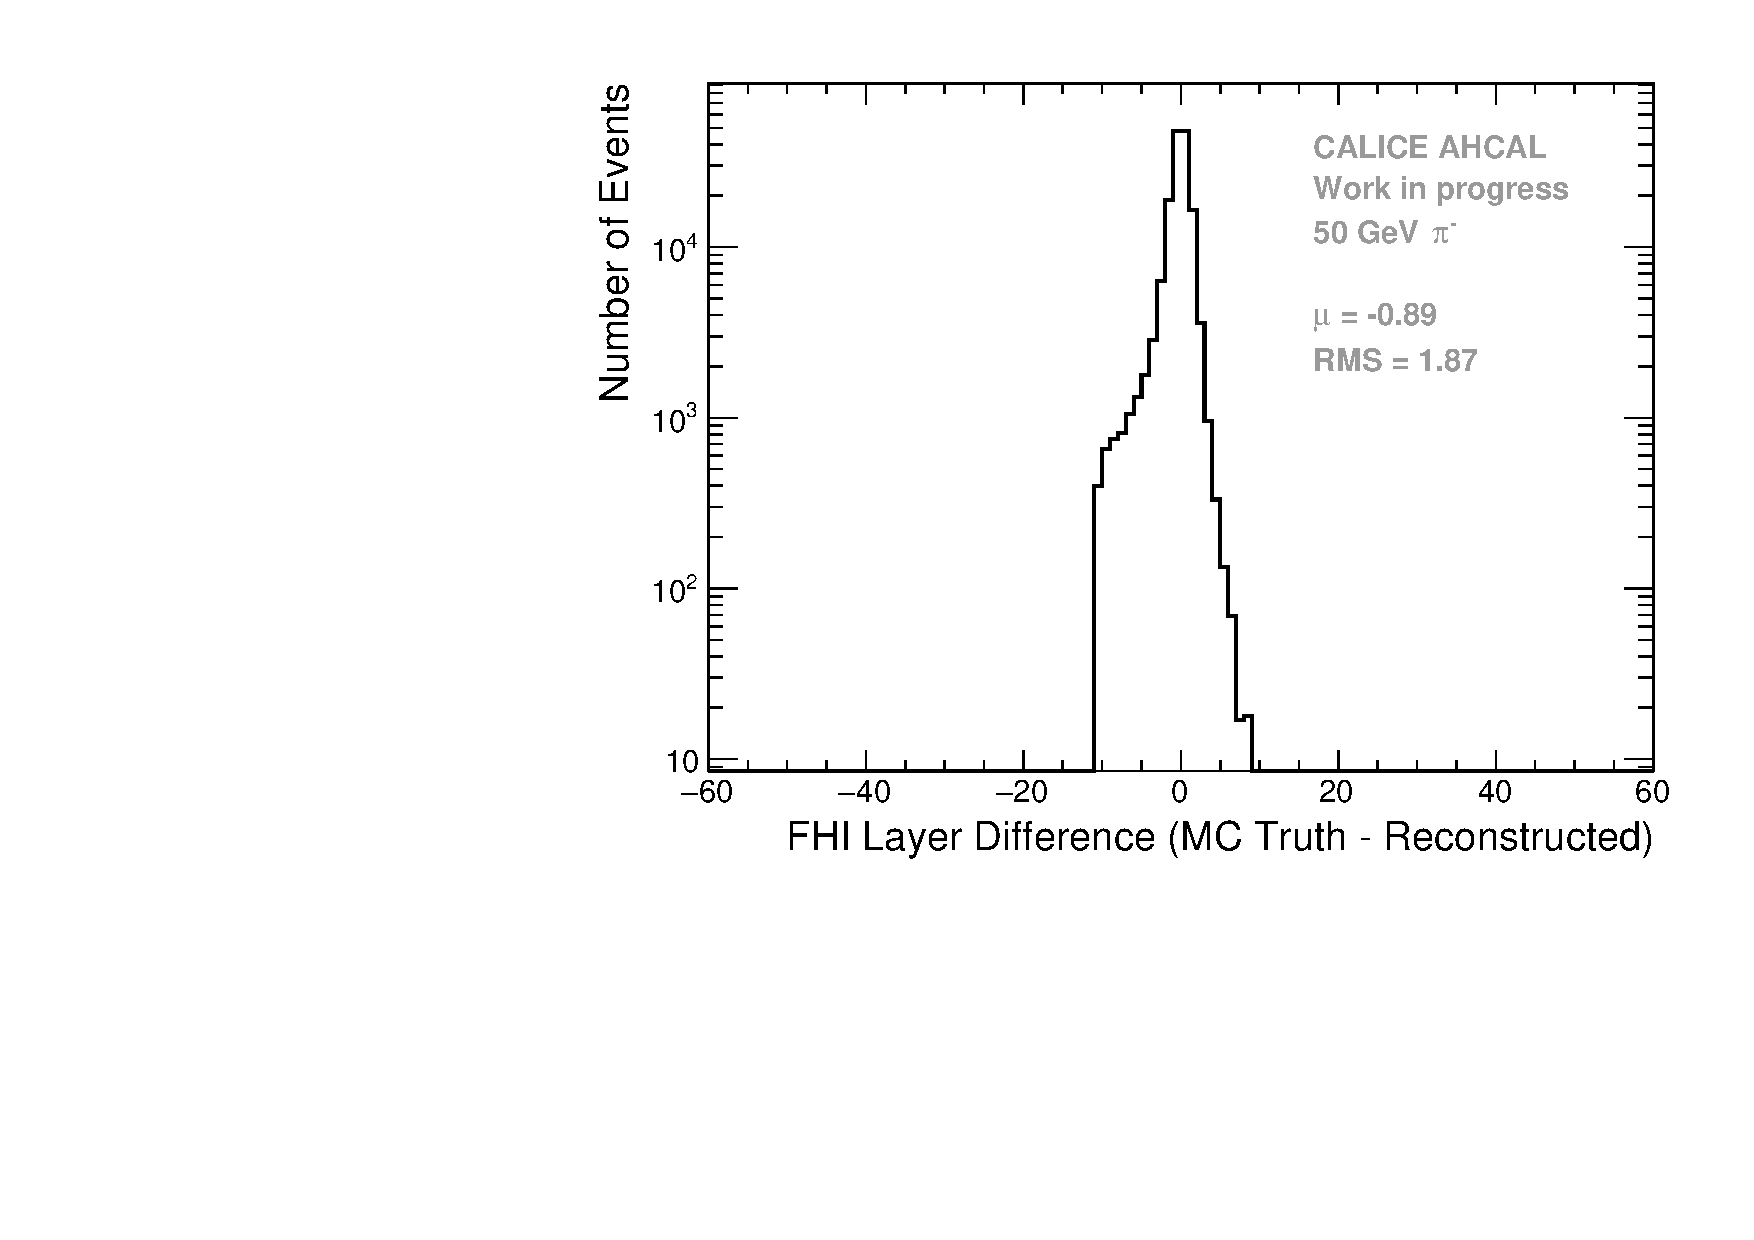
\includegraphics[width=1\textwidth]{../Thesis_Plots/Timing/Pions/Plots/ShowerStart_Difference_noOptimisation.pdf}
		\caption{}\label{fig:Diff_FHI_RecoMC}
	\end{subfigure}
	\hfill
	\begin{subfigure}[t]{0.5\textwidth}
		\centering
		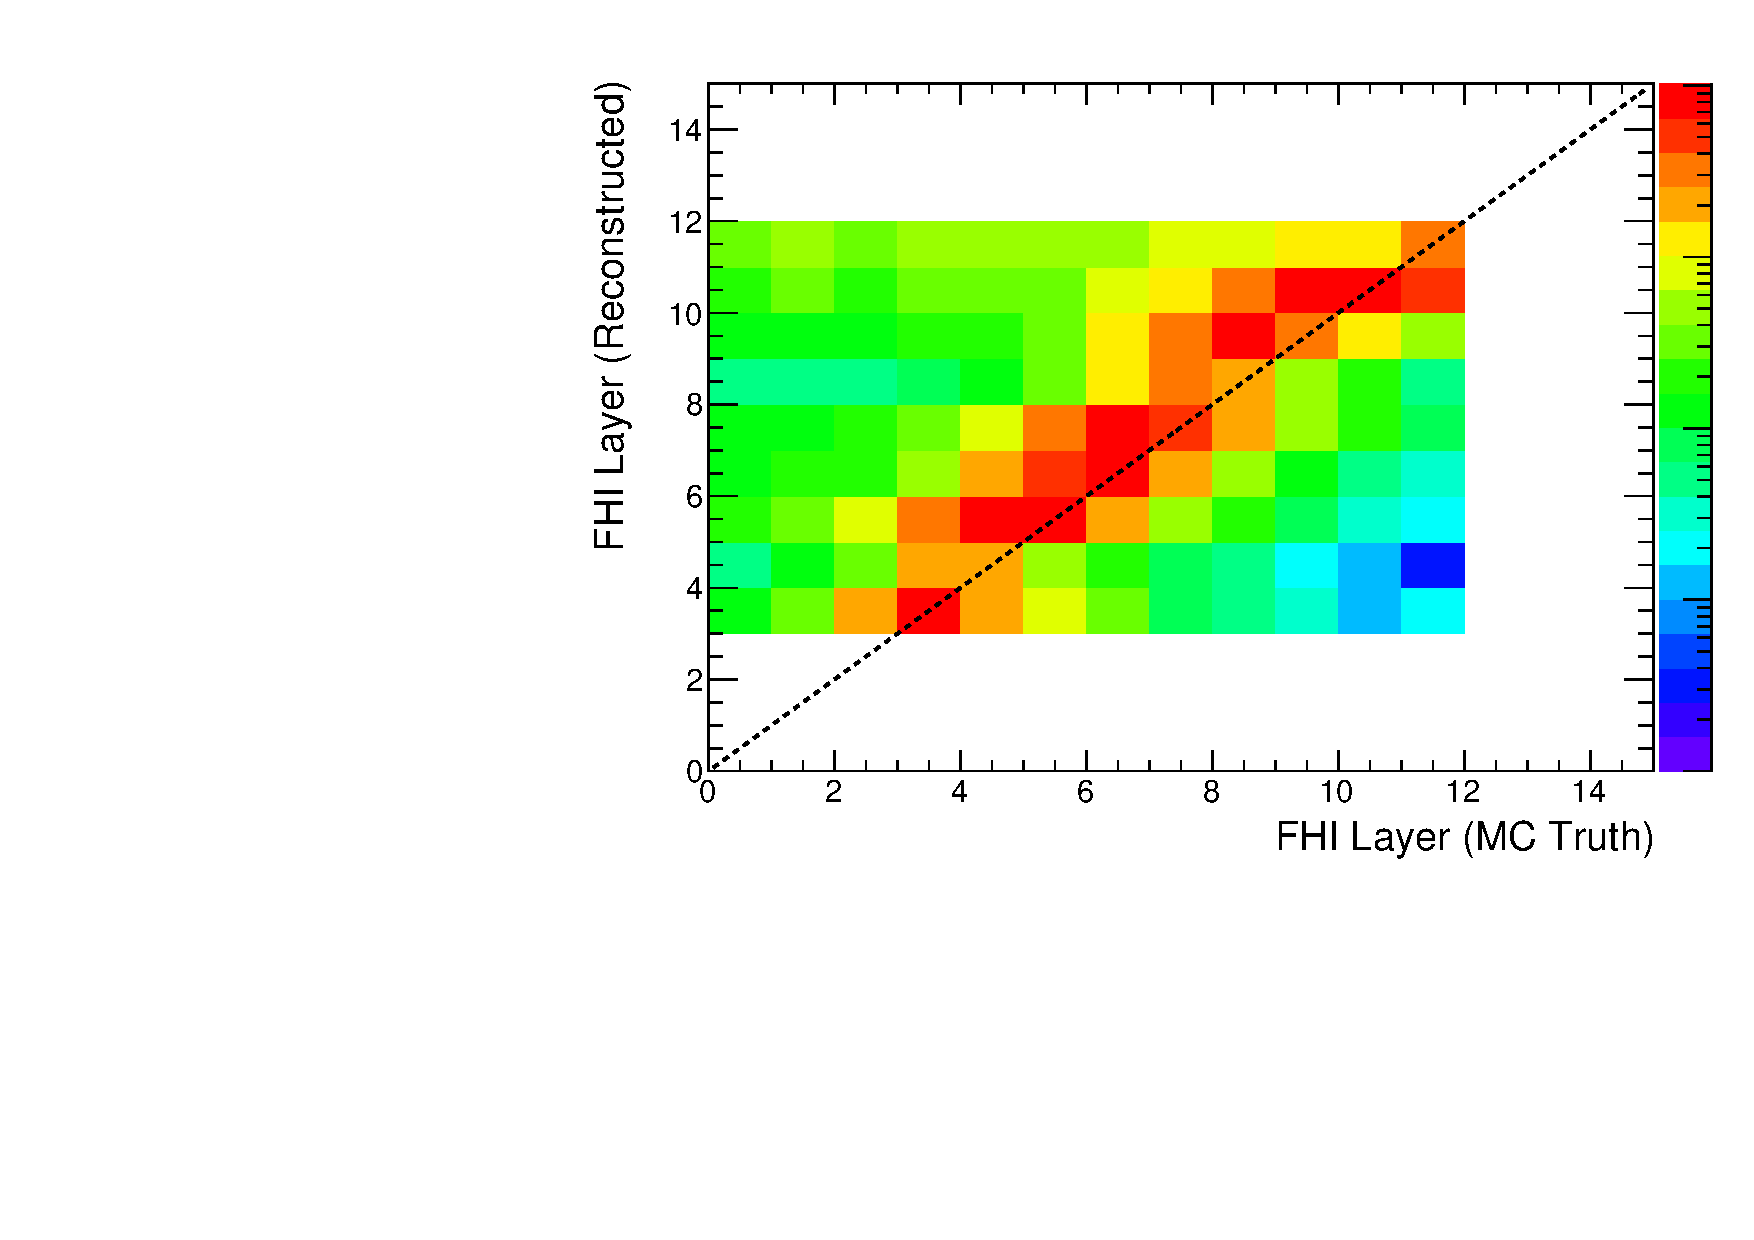
\includegraphics[width=1\textwidth]{../Thesis_Plots/Timing/Pions/Plots/ShowerStart_Difference_noOptimisation_2D.pdf}
		\caption{}\label{fig:Corr_FHI_RecoMC}
	\end{subfigure}
	\caption{Performance of the FHI algorithm in the AHCAL detector. The left plot shows the difference between the reconstructed FHI layer and the MC truth. The distribution is slightly de-centered at -0.81 with a RMS of 1.87. The right plot shows the correlation between the reconstructed FHI layer and the MC truth. The black line represent a guide for a perfect correlation.}
	\label{fig:FHIAlgo}
\end{figure}

It is expected that at a constant distance between the reconstructed FHI layer and the layer investigated that there will be the same dependence of the mean time of the hit as function of the hit distance to the shower axis as the same part of the shower is sampled. Or that inversely, looking at a fixed layer, the expected behavior would be a change in the slope of the mean time of first hit as function of the hit distance to the shower axis for different FHI layer. The figures \ref{fig:Radius_FHI} and \ref{fig:Radius_FHI_Fixed} is an attempt at this.

\begin{figure}[htbp!]
	\begin{subfigure}[t]{0.5\textwidth}
		\centering
		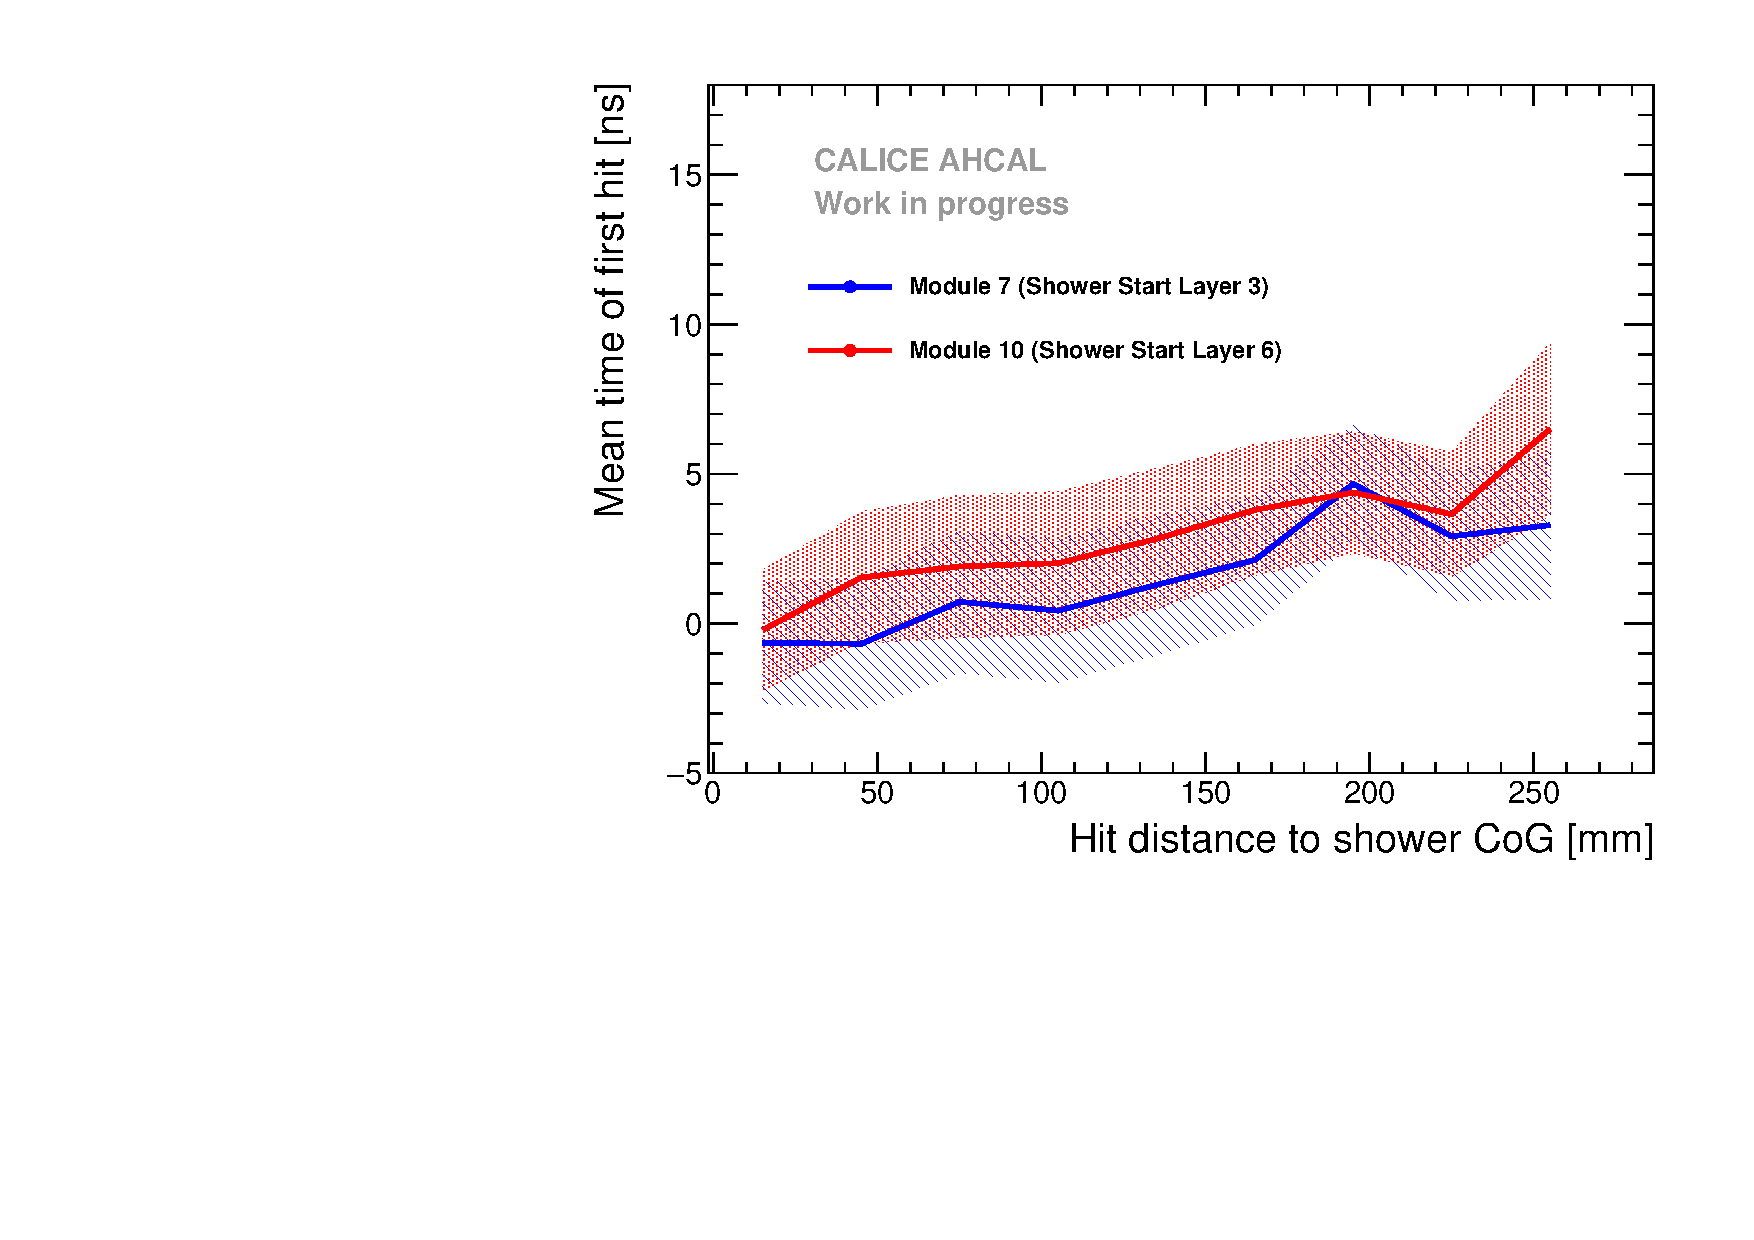
\includegraphics[width=1\textwidth]{../Thesis_Plots/Timing/Pions/Plots/Timing_Radius_Comparison_ShortAsymRange_ShowerStart.pdf}
		\caption{}\label{fig:Radius_FHI}
	\end{subfigure}
	\hfill
	\begin{subfigure}[t]{0.5\textwidth}
		\centering
		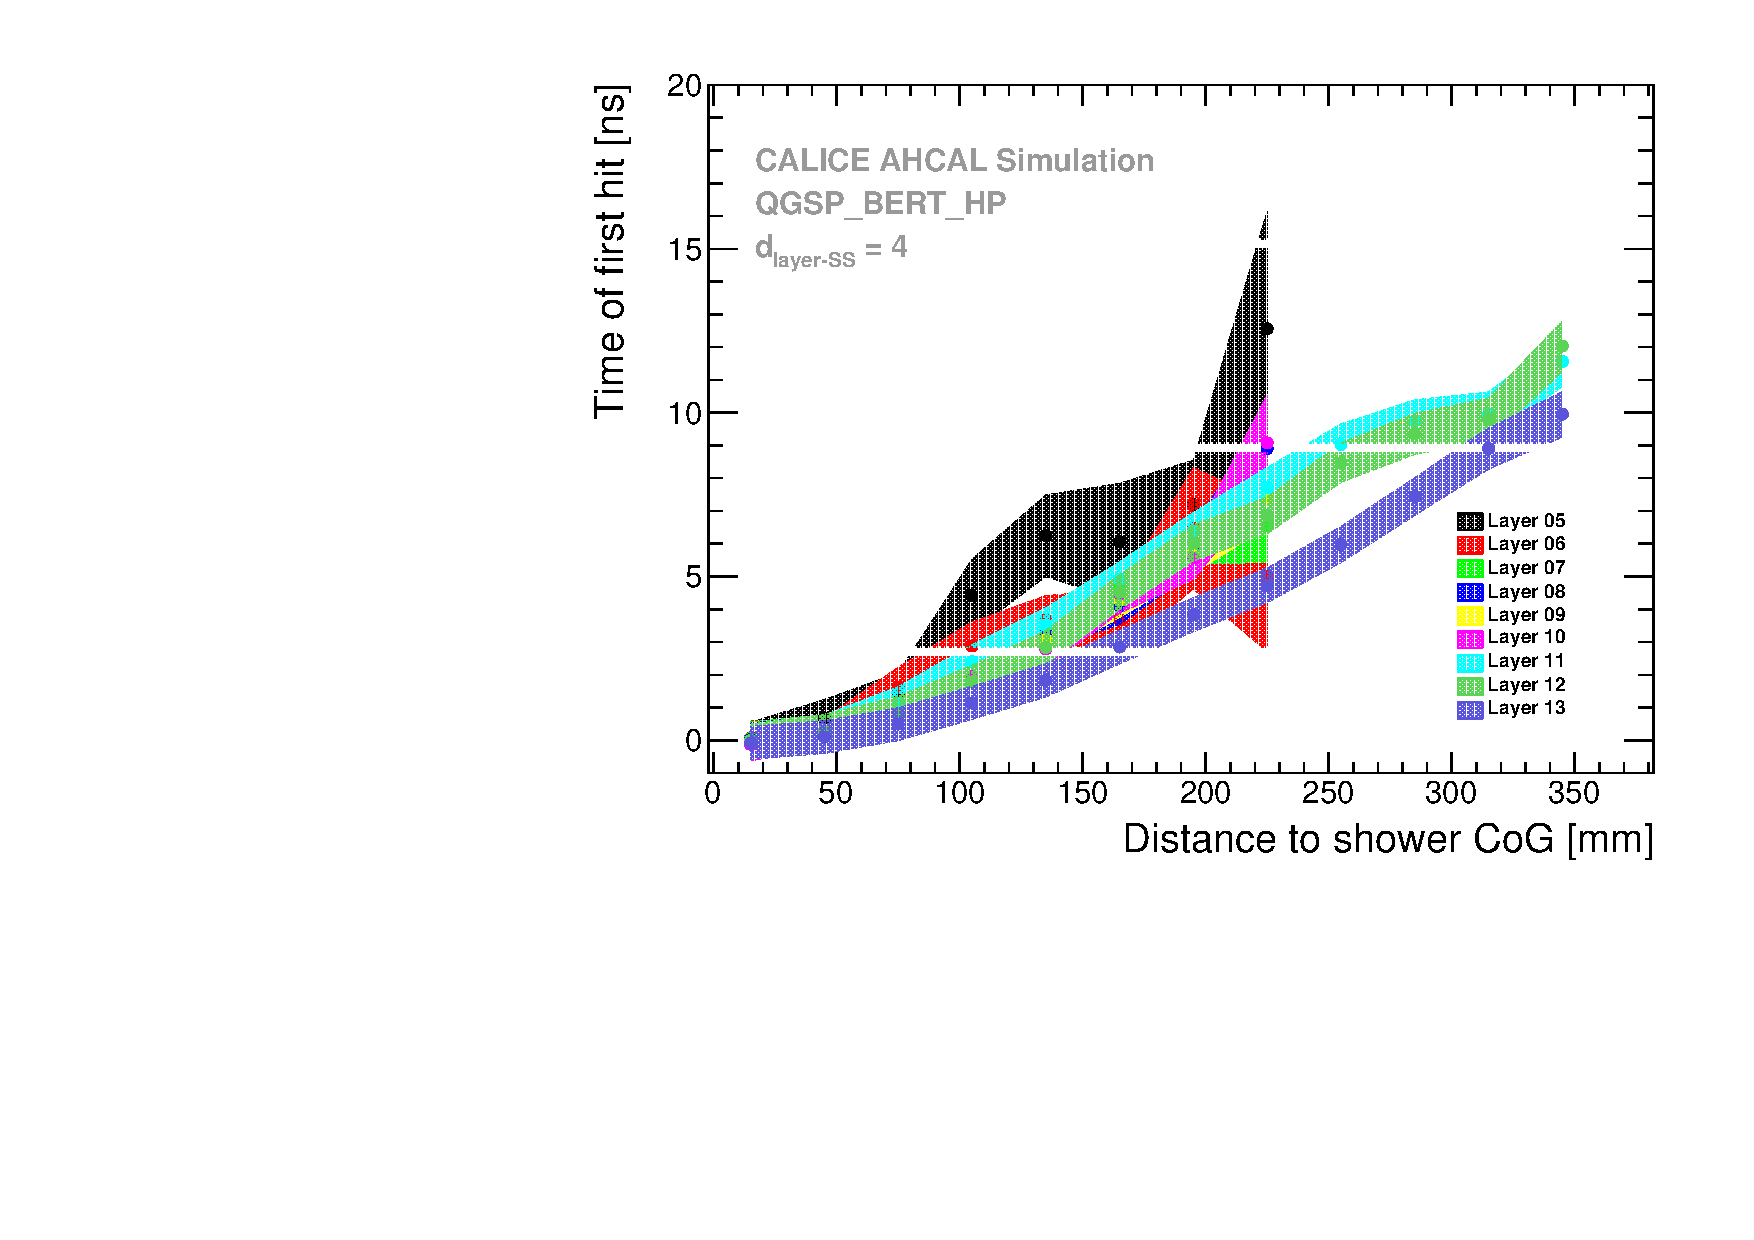
\includegraphics[width=1\textwidth]{../Thesis_Plots/Timing/Pions/Plots/Radius_ShowerStartTruth.pdf}
		\caption{}\label{fig:Radius_FHISim1}
	\end{subfigure}
	\caption{Mean time of first hit as a function of the hit distance to the shower axis for 50 GeV pions for a fixed distance of 4 between the reconstructed FHI layer and the layer investigated. The left plot shows the radial timing profile of layer 7 and 10 in data. The right plots shows the radial timing profile for different layers in simulation with QGSP\_BERT\_HP.}
	\label{fig:Radius_FHIAll}
\end{figure}

The data shows that by fixing the distance between the reconstructed FHI layer and the layer investigated, the mean time of first hit displays the same slope within the systematic uncertainties. On the other hand, by looking at a fixed layer which is in this case the layer 10, it seems that there is a trend of an increase of the curve slope as a function of the reconstructed FHI layer within the systematics. But because of many layers not working well, it is difficult to find a comparable configuration to confirm the observation. As well, a reduction of the systematic uncertainty is needed. This has been checked in simulation with QGSP\_BERT\_HP as shown in figures \ref{fig:Radius_FHISim1} and \ref{fig:Radius_FHI_FixedSim}. The simulation agrees well with the observation made in the data.

\begin{figure}[htbp!]
	\begin{subfigure}[t]{0.5\textwidth}
		\centering
		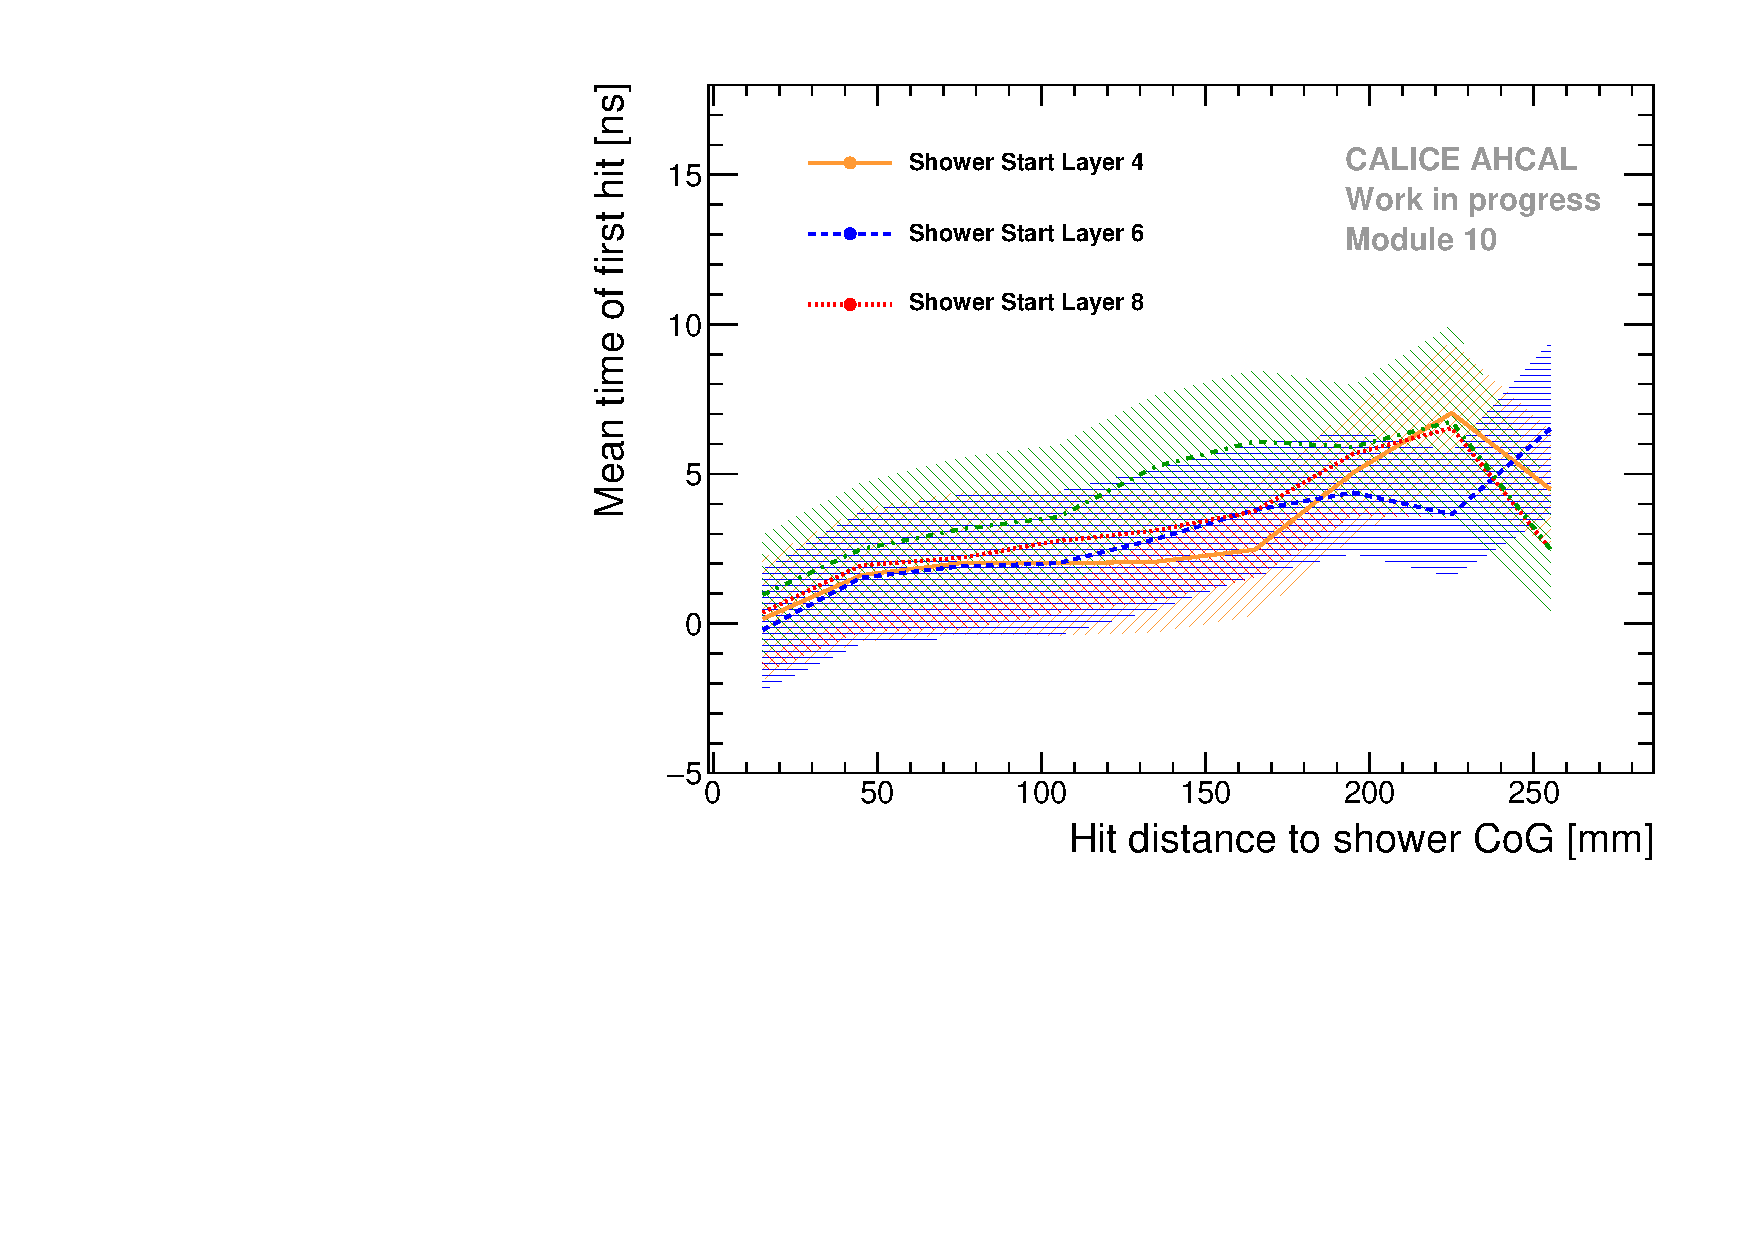
\includegraphics[width=1\textwidth]{../Thesis_Plots/Timing/Pions/Plots/Timing_Radius_Comparison_ShortAsymRange_ShowerStart_FixedModule.pdf}
		\caption{}\label{fig:Radius_FHI_Fixed}
	\end{subfigure}
	\hfill
	\begin{subfigure}[t]{0.5\textwidth}
		\centering
		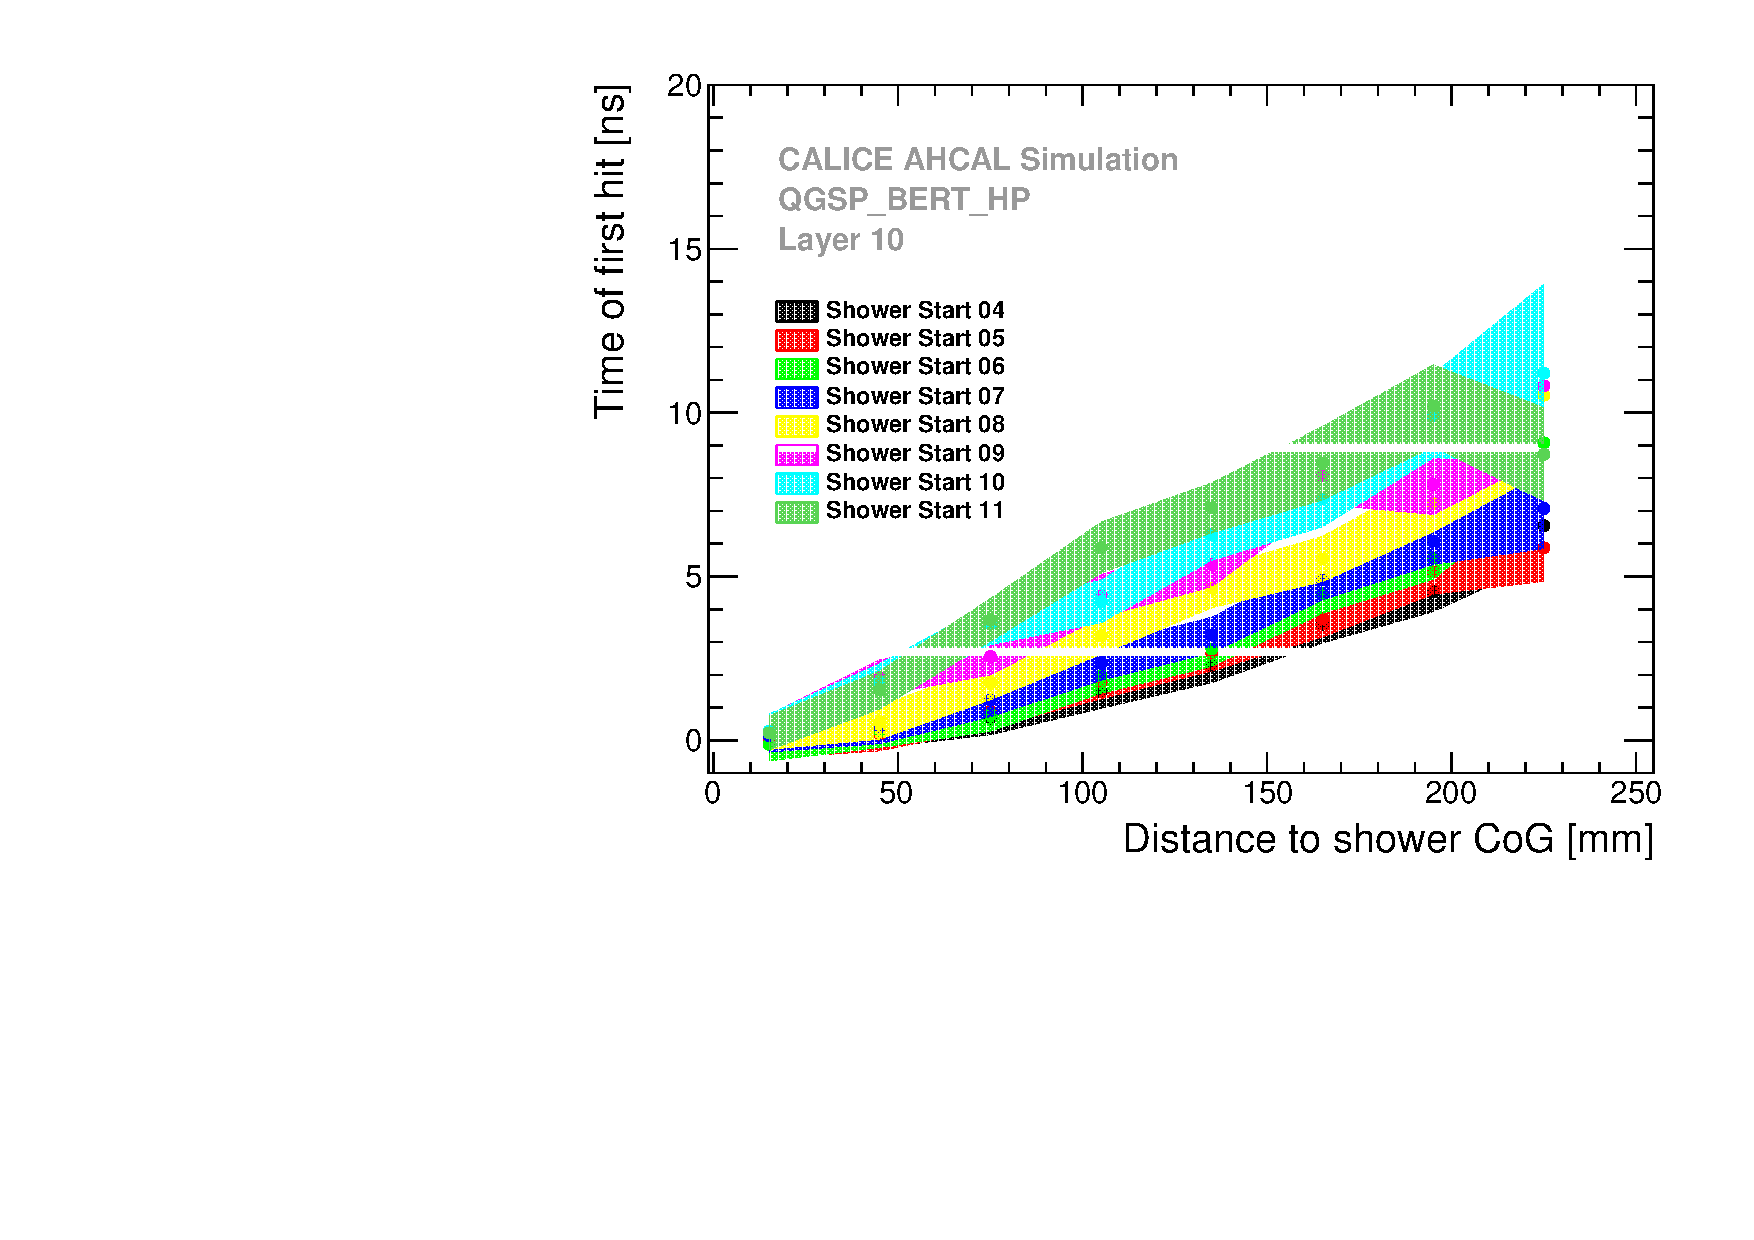
\includegraphics[width=1\textwidth]{../Thesis_Plots/Timing/Pions/Plots/Radius_ShowerStartTruth_FixedModule.pdf}
		\caption{}\label{fig:Radius_FHI_FixedSim}
	\end{subfigure}
	\caption{Mean time of first hit as a function of the hit distance to the shower axis for 50 GeV pions for different reconstructed FHI layer. In data on the left and in simulation with QGSP\_BERT\_HP on the right.}
	\label{fig:Radius_FHISim}
\end{figure}

\subsection{Longitudinal dependence of timing profiles}

Hadronic showers develop as well longitudinally, therefore the longitudinal dependence of mean time of the first hit as a function of the layer position was investigated. It is expected that the further you are in the calorimeter that more low energy neutrons contribute to the energy deposition thus enhancing the late tail. The figure \ref{fig:Depth_Comparison} shown the mean time of first hit as function of the layer position for muon, electron and pion beams.

\begin{figure}[htbp!]
	\begin{subfigure}[t]{0.5\textwidth}
		\centering
		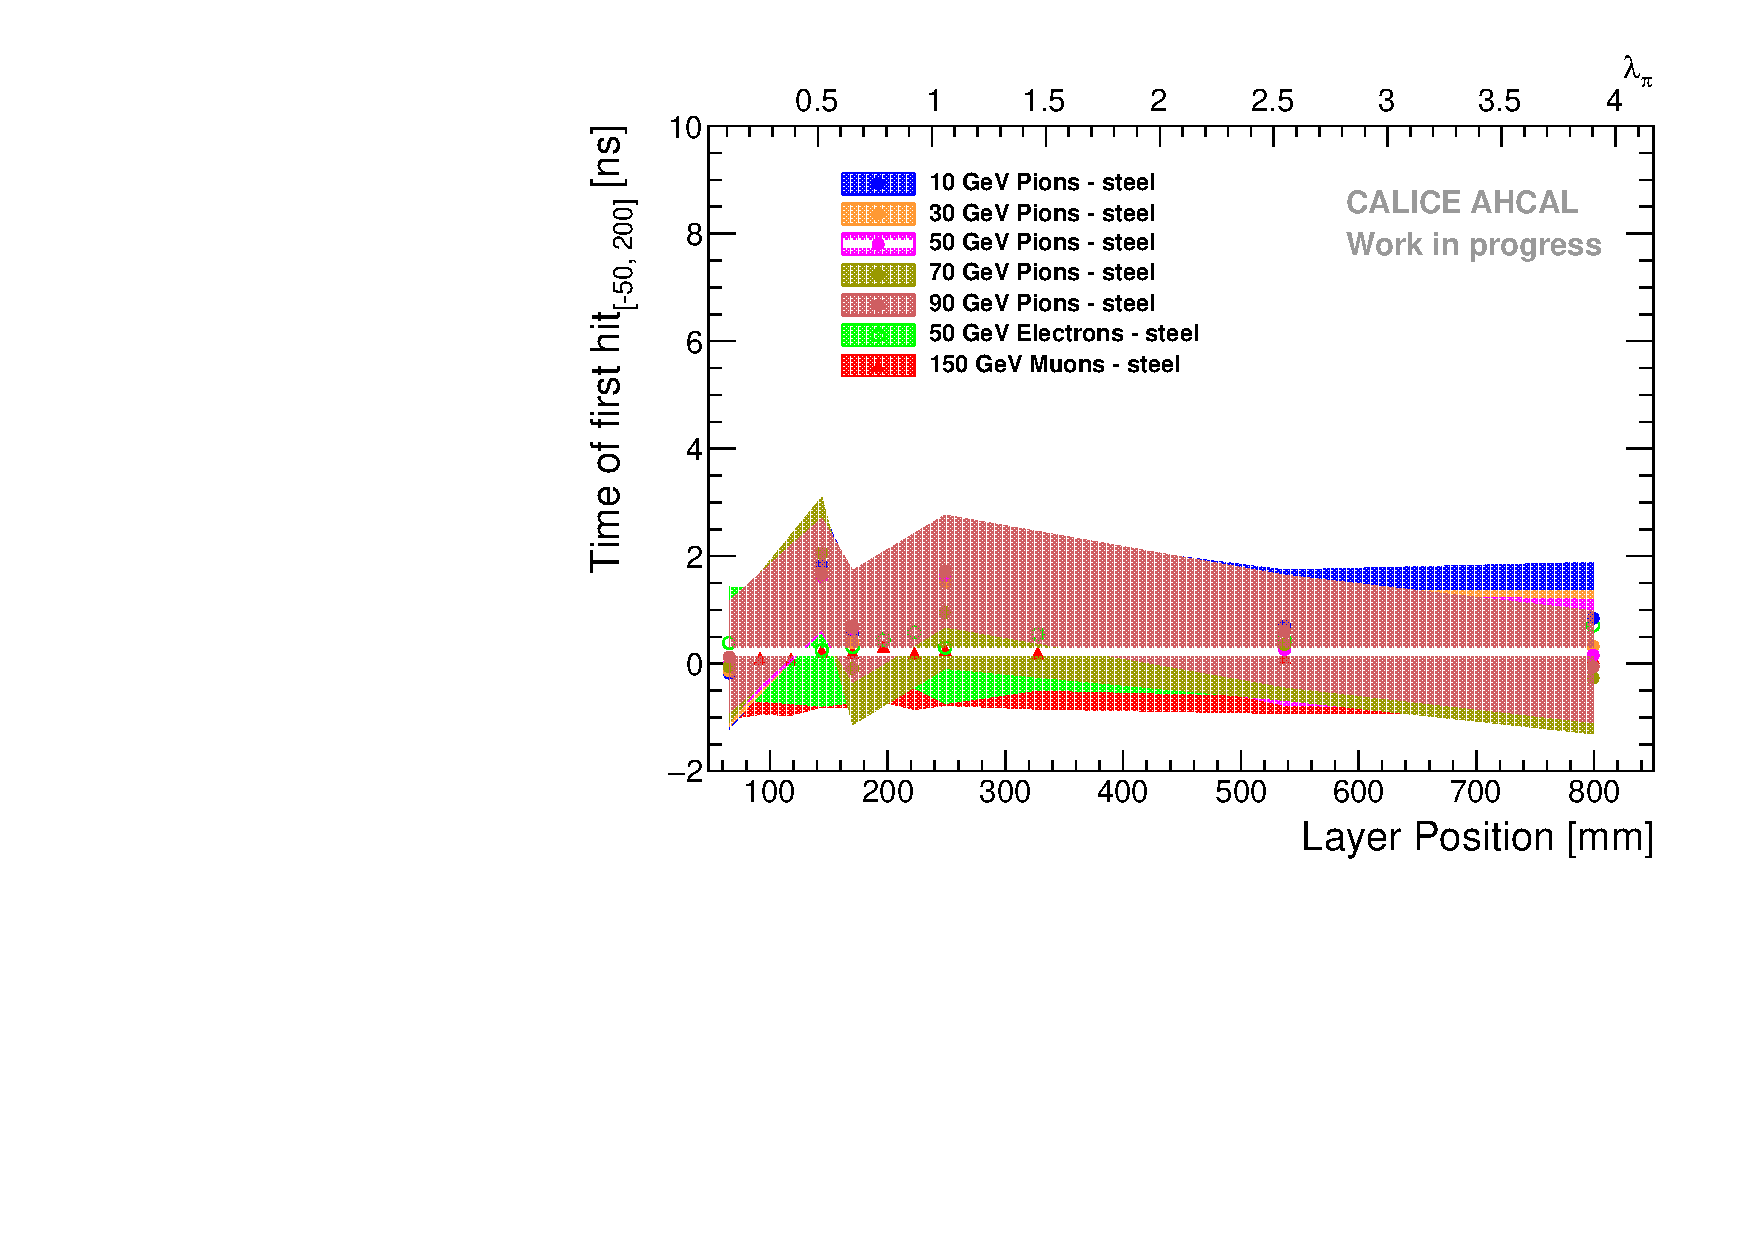
\includegraphics[width=1\textwidth]{../Thesis_Plots/Timing/Pions/Plots/Timing_Depth_Comparison_ShortAsymRange.pdf}
		\caption{} \label{fig:Depth_Comparison}
	\end{subfigure}
	\hfill
	\begin{subfigure}[t]{0.5\textwidth}
		\centering
		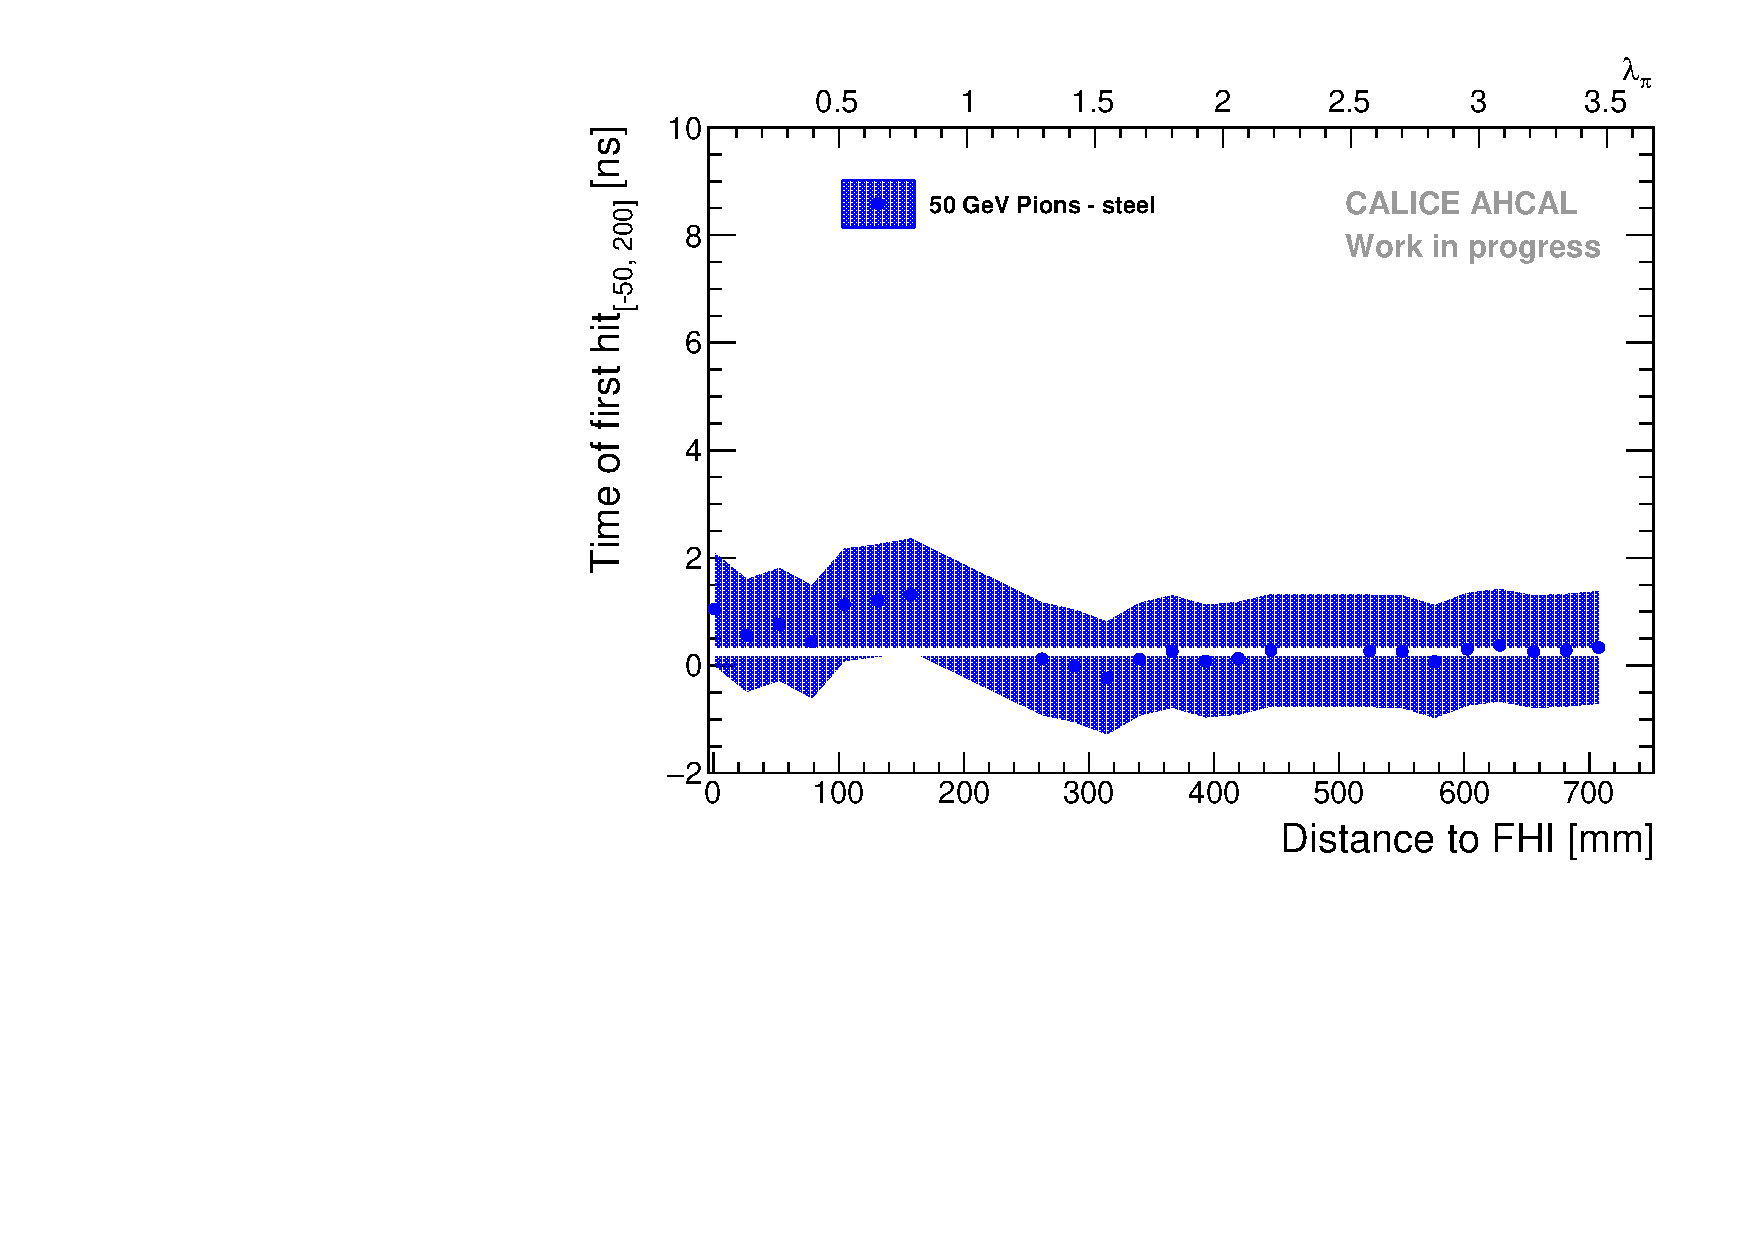
\includegraphics[width=1\textwidth]{../Thesis_Plots/Timing/Pions/Plots/Timing_Depth_Comparison_ShortAsymRange_ShowerStart.pdf}
		\caption{}\label{fig:Depth_Comparison_FHI}
	\end{subfigure}
	\caption{The left plot shows the longitudinal timing profile as a function of the layer position for muon, electron and pion beams. The right plot shows the longitudinal timing profile as a function of the distance to the reconstructed FHI layer for 50 GeV pions.}
	\label{fig:DepthProfile}
\end{figure}

In data, no increase of the mean time is observed as a function of the layer depth as well no energy dependence is visible. This may be because the sensitivity to the late component is suppressed by the time resolution of the calorimeter and the size of the systematic errors. An attempt was made to get a better sensitivity by looking at the mean time of first hit as function of the distance to the reconstructed FHI layer as shown in figure \ref{fig:Depth_Comparison_FHI}. However, the figure still shows a flat distribution centered around 0 ns.

The longitudinal timing profile was also compared to simulations. The mean time of first hit is compatible with a flat distribution around 0 ns for all models. The timing resolution of the AHCAL may be too high in order to be sensitive to any small changes of the mean time over the calorimeter depth. The simulation with QGSP\_BERT\_HP without time smearing is shown in figure \ref{fig:Depth_Sim_noSmearing}. It shows that there is an increase of the mean time of first hit as function of the layer in the order of 1 ns and confirms that due to the electronics time resolution this is not visible in data.

\begin{figure}[htbp!]
	\begin{subfigure}[t]{0.5\textwidth}
		\centering
		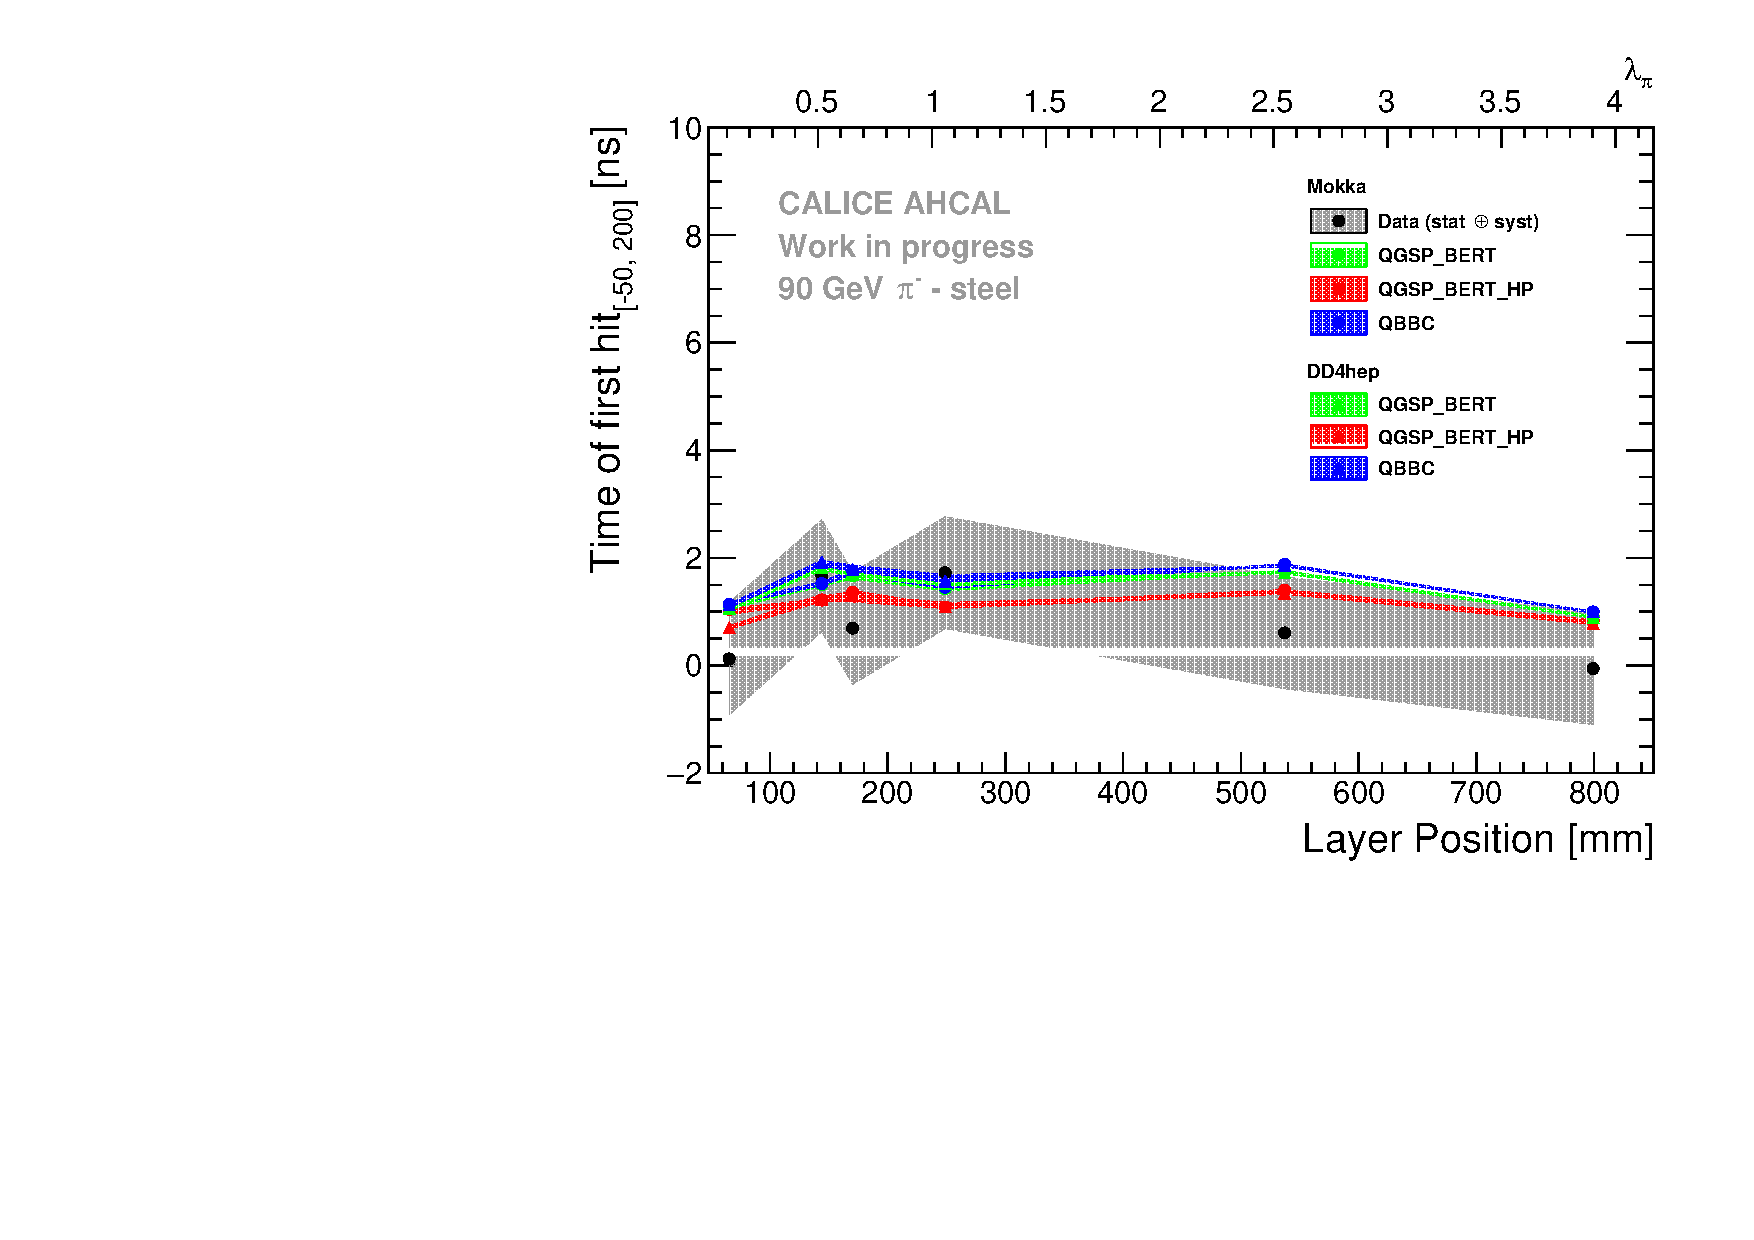
\includegraphics[width=1\textwidth]{../Thesis_Plots/Timing/Pions/Plots/ComparisonToSim/Time_Depth_90GeV.pdf}
		\caption{} \label{fig:Depth_SimData_Comparison}
	\end{subfigure}
	\hfill
	\begin{subfigure}[t]{0.5\textwidth}
		\centering
		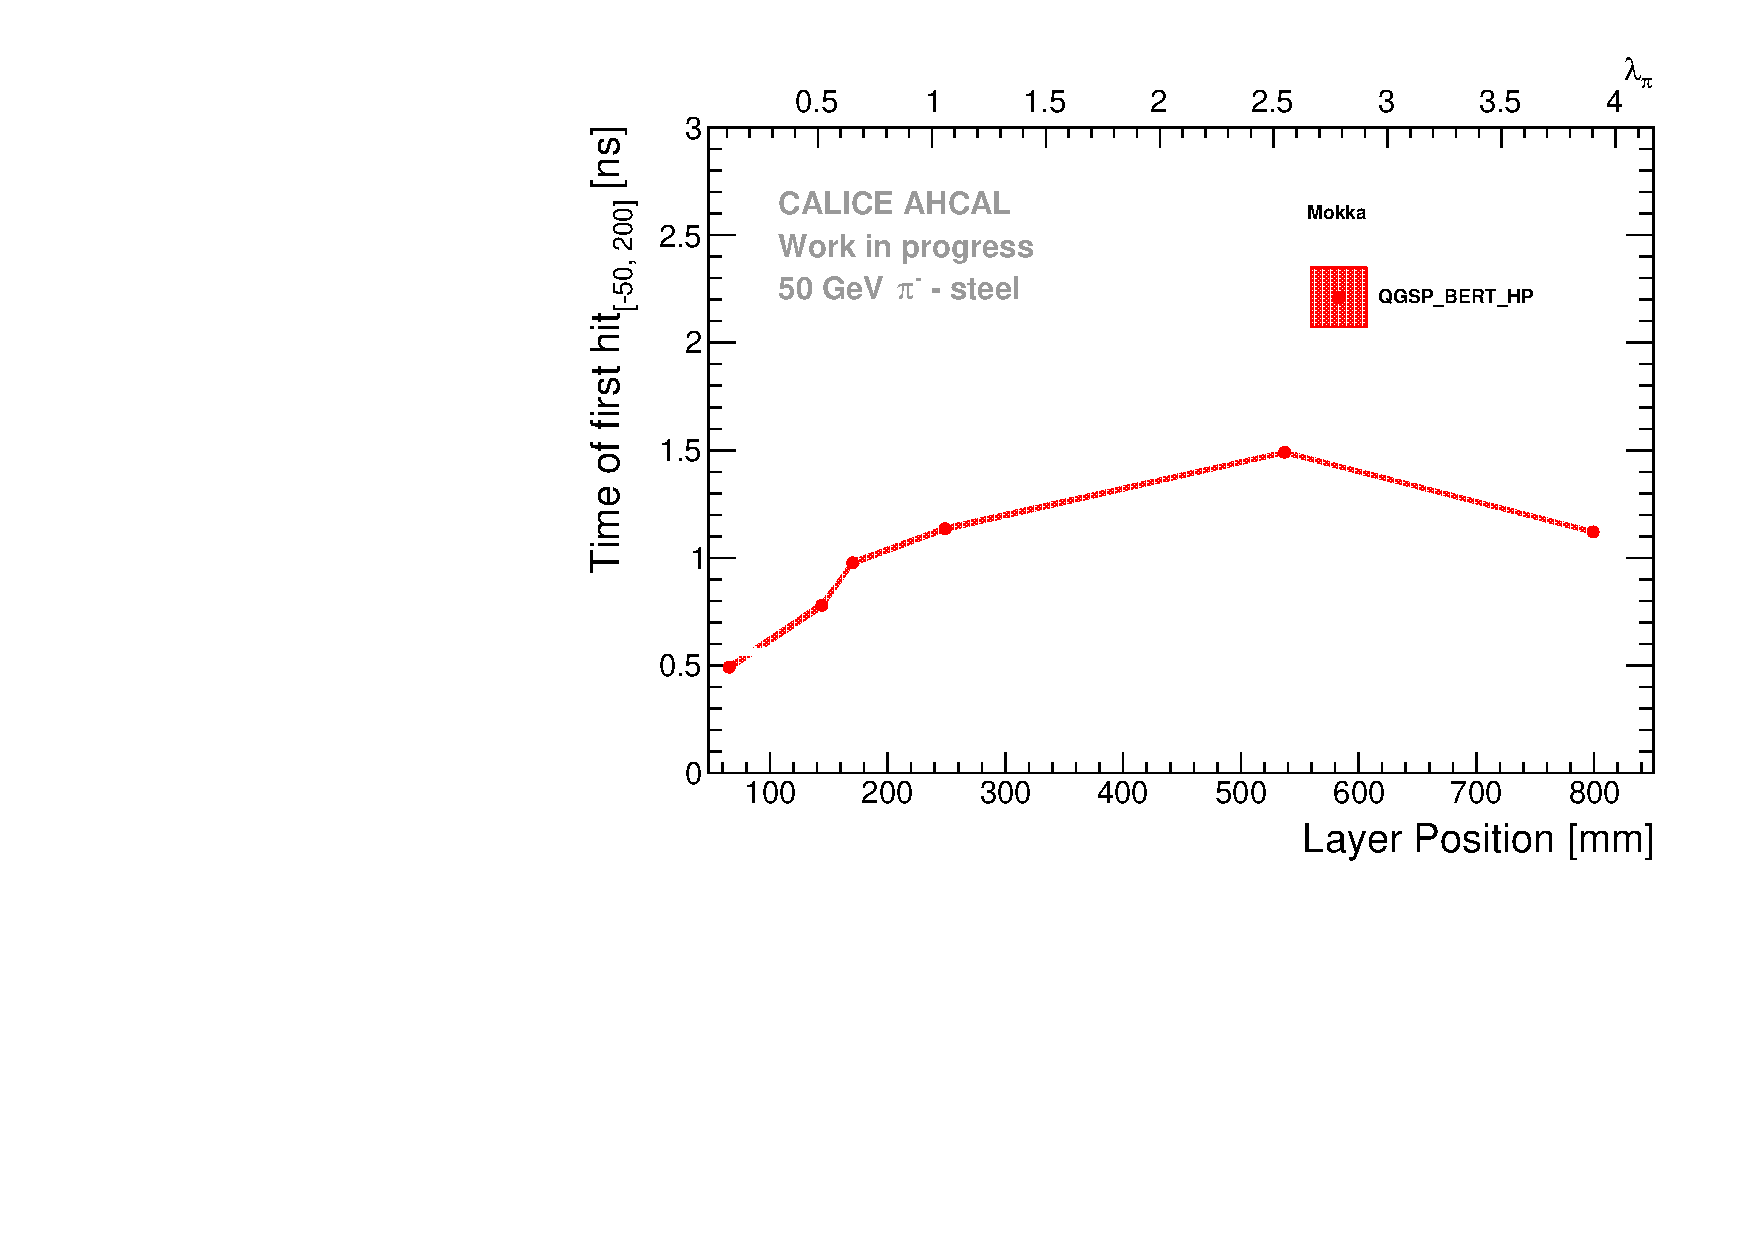
\includegraphics[width=1\textwidth]{../Thesis_Plots/Timing/Pions/Plots/Time_Depth_50GeV_QGSP_BERT_HP_noSmearing.pdf}
		\caption{}\label{fig:Depth_Sim_noSmearing}
	\end{subfigure}
	\caption{On the left, comparison of the time of first hit as a function of the layer position in data and simulation for 90 GeV pions. The grey and color bands shows the systematics. On the right, time of first hit as function of the layer position for 50 GeV pions in simulation with the QGSP\_BERT\_HP physics list with no time smearing.}
\end{figure}

\subsection{Time correlations between layers}

The advantage of this studied prototype over T3B is the possibility to investigate time correlations between layers. For this study, the data below 50 ns is ignored as only the tail of the timing distributions is interesting.

The procedure is done by looking at each hit in layer $i$ and checking in layer $i+1$ for a hit within a distance of 60 mm in the $x:y$ plane. If a hit is found, both times are plotted against each other. If more than one hit is found in layer $i+1$ within a distance of 60 mm, the closest in the $x:y$ plane is taken.

Two types of correlations were investigated, short and long. For the short correlation, the layers 6 and 7 were chosen, corresponding to 1 $X_0$ or 0.1 $\lambda_{\pi}$. As for the long, the layers 13 and 14 were selected, corresponding to 10 $X_0$ or 1 $\lambda_{\pi}$. These were chosen due to the fact that few layers were working properly. It is expected that EM sub-showers can lead to a correlation of hit times for the layers 6 and 7, while the layers 13 and 14 are far apart, and therefore would show less correlation of hit times. The hit times correlation is shown in figure \ref{fig:TimeCorrelation} for the 50 GeV dataset.

\begin{figure}[htbp!]
	\begin{subfigure}[t]{0.5\textwidth}
		\centering
		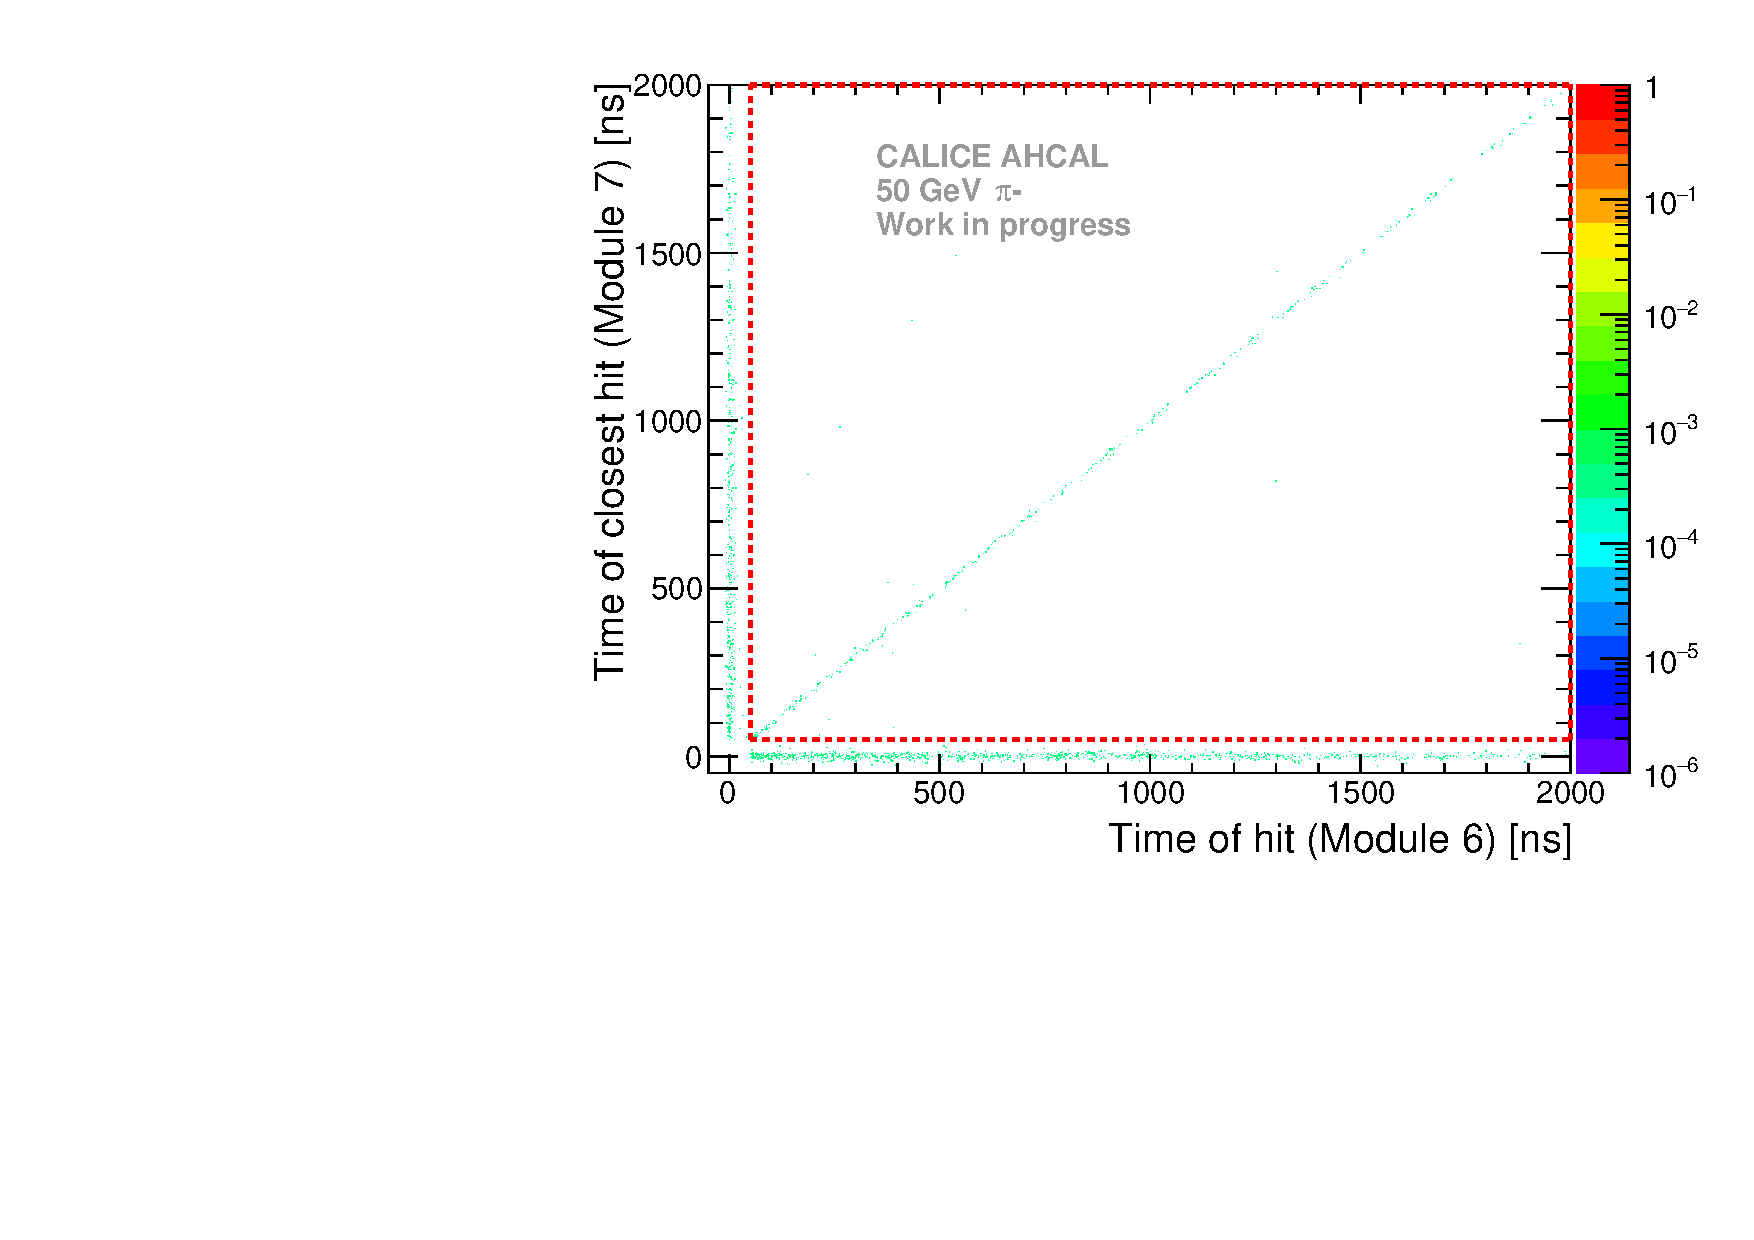
\includegraphics[width=1\textwidth]{../Thesis_Plots/Timing/Pions/Plots/Time_Correlation_short.pdf}
		\caption{} \label{fig:Time_Corr_short}
	\end{subfigure}
	\hfill
	\begin{subfigure}[t]{0.5\textwidth}
		\centering
		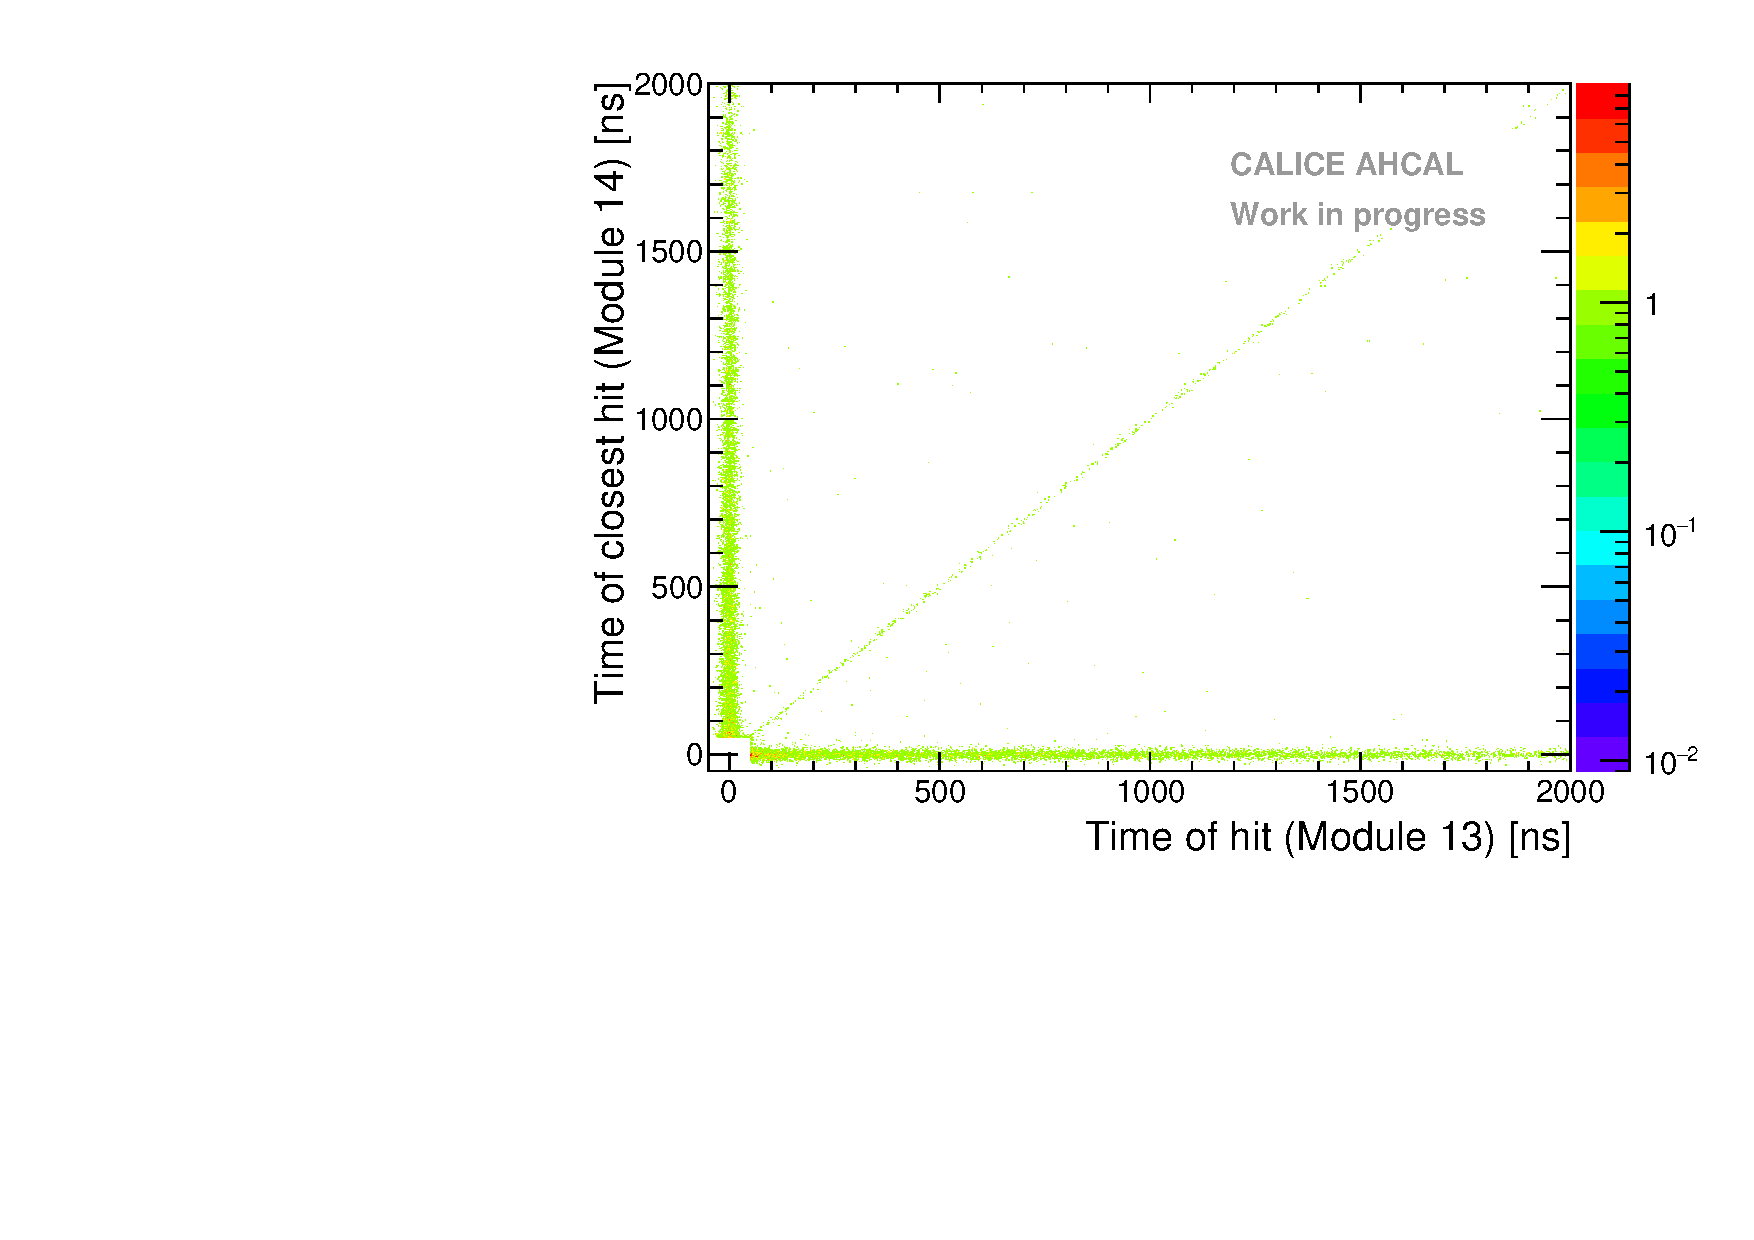
\includegraphics[width=1\textwidth]{../Thesis_Plots/Timing/Pions/Plots/Time_Correlation_long.pdf}
		\caption{}\label{fig:Time_Corr_long}
	\end{subfigure}
	\caption{The left plot shows the time correlation between layer 6 and 7 separated by 1 $X_0$. The right plot shows the time correlation for layers 13 and 14 separated by 1 $\lambda_{\pi}$. Each bin is normalized to the number of entries in the 2D histogram. The red box represent the region of interest. Both plots show a visible time correlation.}
	\label{fig:TimeCorrelation}
\end{figure}

The figures show that a correlation is visible in the data for both cases. To quantify this, the following ratio is calculated
\begin{equation}\label{eq:CorrelCalcul}
	R = \frac{\int_{50 ns}^{2 \mu s} \int_{50 ns}^{2 \mu s} \frac{dN_i(t)}{dt_i} \frac{dN_j(t)}{dt_j} dt_i dt_j}{N_{tot}}
\end{equation}
where N$_{tot}$ is the total number of entries in the histogram and the nominator is the number of entries between 50 ns and \SI{2}{\micro\second} in the red box of the above figures.

The results show that 18.19\% of the entries are in the red box region for the short correlation. This may come from EM sub-showers in the hadron shower. For the long correlation, 3.24\% of the entries are in the red box region. This represents a substantial amount of hits that are correlated.

\begin{figure}[htbp!]
	\begin{subfigure}[t]{0.5\textwidth}
		\centering
		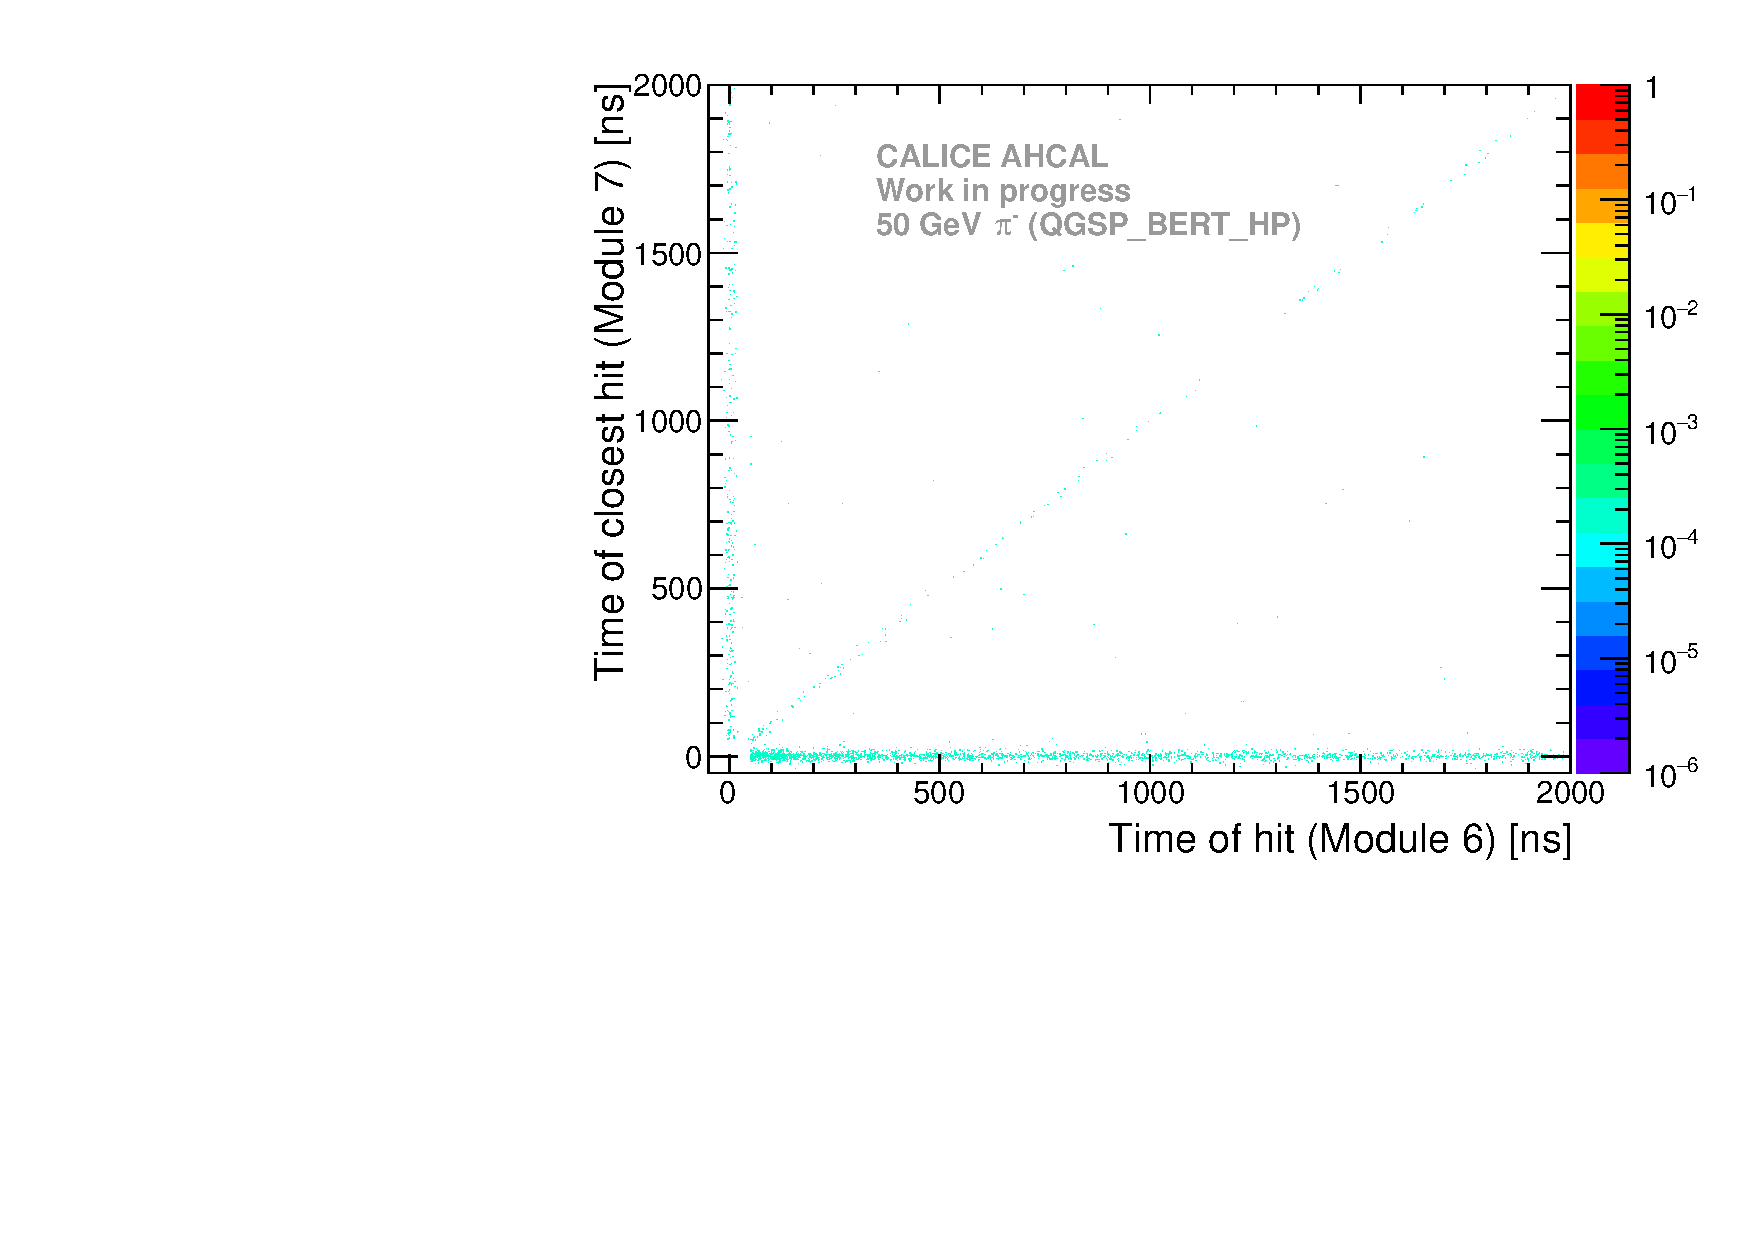
\includegraphics[width=1\textwidth]{../Thesis_Plots/Timing/Pions/Plots/ComparisonToSim/Time_Correlation_50GeV_short_QGSPBERTHP.pdf}
		\caption{Short correlation (QGSP\_BERT\_HP).} \label{fig:Corr_short_QGSPBERTHP}
	\end{subfigure}
	\hfill
	\begin{subfigure}[t]{0.5\textwidth}
		\centering
		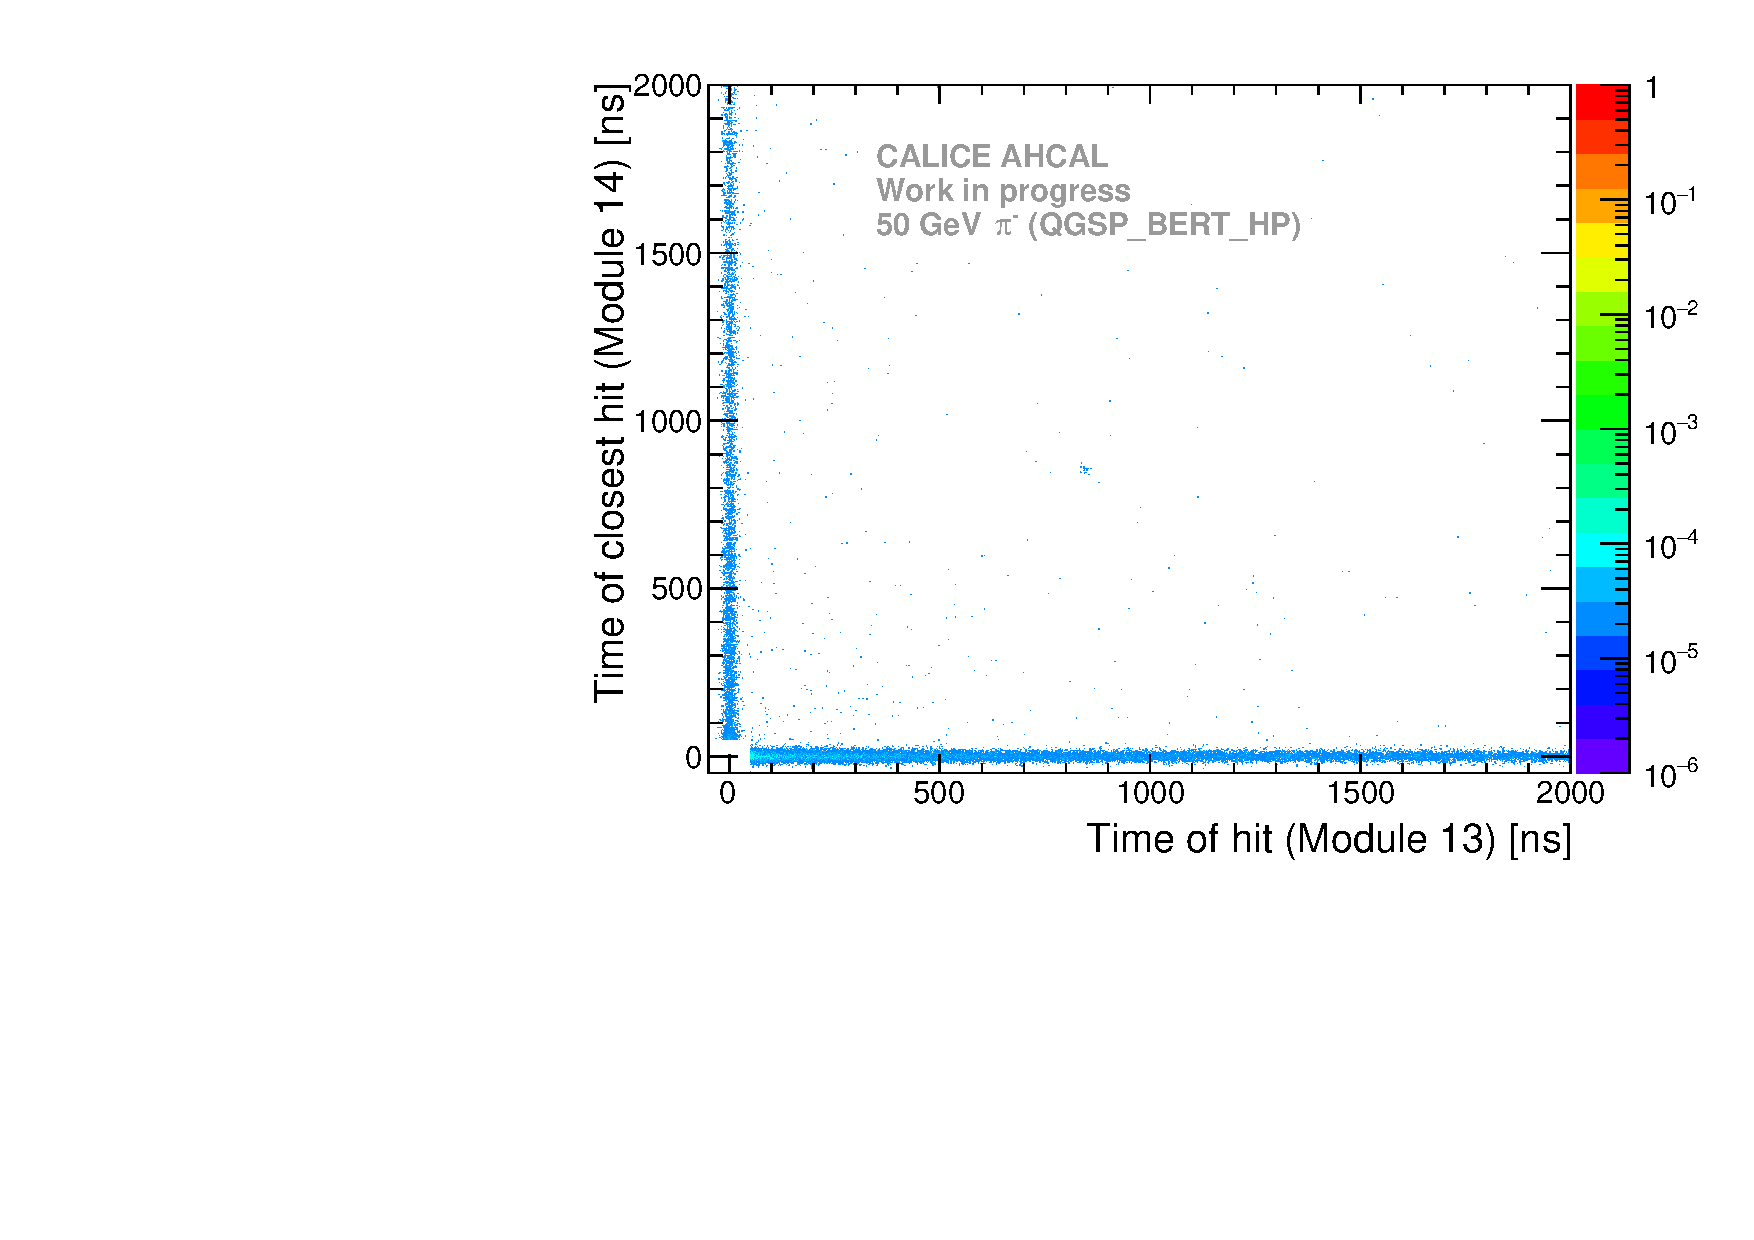
\includegraphics[width=1\textwidth]{../Thesis_Plots/Timing/Pions/Plots/ComparisonToSim/Time_Correlation_50GeV_long_QGSPBERTHP.pdf}
		\caption{Long correlation (QGSP\_BERT\_HP).} \label{fig:Corr_long_QGSPBERTHP}
	\end{subfigure}
	\caption{Hit timing correlations between layers 6 and 7 and layers 13 and 14 in the \mokka simulation with QGSP\_BERT\_HP for 50 GeV pions. Each bin is normalized to the total number of entries in the 2D histogram.}
	\label{fig:Corr_Mokka_Simulation}
\end{figure}

This was compared to simulation using the QGSP\_BERT\_HP physics lists as shown in figures \ref{fig:Corr_Mokka_Simulation}. The figures for simulations with other physics lists can be seen in appendix \ref{appendix:TimingAdd}. In the same way, the number of correlated time hits was calculated and it is summarized in table \ref{table:Correlation_DataSim}. Looking at the numbers, there is a large discrepancy between data and simulation. In general, the simulation possesses less correlated hits than in data for both type of correlations. In addition, the \ddhep simulation has slightly less correlated hits, around 1\%, at a short range than in the \mokka simulation which is not understood.

\begin{table}[htb!]
	\centering
	\caption{Table with fraction of events in the red box region as calculated with equation \ref{eq:CorrelCalcul}. The top is for \mokka simulations, the bottom is for \ddhep simulations.}
	\label{table:Correlation_DataSim}
	\begin{tabular}{@{} lcc @{}}
		\toprule
		Type & Short correlation [\%] & Long correlation [\%]\\
		\midrule
		\multirow{2}{*}{Data} & \multirow{2}{*}{18.19} & \multirow{2}{*}{3.24}\\ & &\\
		\midrule
		\multirow{2}{*}{QGSP\_BERT} & 3.53 & 0.55\\ & 2.30 & 0.50\\
		\multirow{2}{*}{QGSP\_BERT\_HP} & 3.62 & 0.60\\ & 2.27 & 0.54\\
		\multirow{2}{*}{QBBC} & 3.61 & 0.59\\ & 2.31 & 0.53\\
		\bottomrule
	\end{tabular}
\end{table}

The reason for the discrepancy between data and simulation is not clear though it may come from the selection of the data that may be not good enough to reject multi-particle events as shown figure \ref{fig:DoubleParticleEvent}, therefore providing more correlated hits than observed in simulation. More data, especially with a better detector to be sure to reject multi-particle events, is required in order to understand the origin of such correlations.

\newpage
\section{Summary and Outlook}

The understanding of the time structure of hadronic showers and the level of accuracy reflected in \geant simulations is highly relevant for calorimeters at future (linear) collider experiments. This can be applied for conditions with high level of background such as $\gamma\gamma \rightarrow \text{hadrons}$ or high repetition rates experiments to remove out-of-time pile-up events.

A testbeam at the SPS facility at CERN in July 2015 was focused to address this. The AHCAL technological prototype, close to the ILD detector design, was equipped with 14 layers inserted in a steel absorber and using scintillator tiles as active material readout by SiPMs to provide radial and longitudinal sampling of showers with high granularity and ns-scale time resolution. For the first time, time study of hadronic showers was done on a large scale using integrated readout electronics.\\[0.1cm]

\noindent\textbf{Energy scale calibration:} In chapter \ref{chap:ECalibAHCAL}, the energy scale calibration of the AHCAL was presented. 85\% of the AHCAL detector has been calibrated to a precision of around 1.7\%. Validation studies of the simulation concluded that the a good average energy calibration is achieved at the cell level. In addition, the simulation has been further validated with electromagnetic showers showed that the data is reproduced at a level of 10-20\%.\\[0.1cm]

\noindent\textbf{Timing calibration:} In chapter \ref{chap:TimingCalib}, the time calibration procedure of the AHCAL was presented. More than 20000 constants have been determined from data. A time resolution of the order of 5 ns is achieved in a muon beam.\\[0.1cm]

\noindent\textbf{Validation of the calibration:} In chapter \ref{chap:TimingValidation}, the timing calibration was cross-checked with the electron dataset and the timing simulation has been validated. Due to an effect of the readout electronics, the time resolution for electron is worse, with a value between 7.5 to 8.2 ns depending on the beam energy. The simulation reproduces the data within an acceptable level of 10-20\%, however the tails of the time distribution are not well reproduced due an imperfect implementation of noise hits.\\[0.1cm]

\noindent\textbf{Timing of hadron showers:} In chapter \ref{chap:TimingPions}, the timing of hadronic showers was studied. The data shows that late energy depositions are concentrated at low hit energies below 1 MIP in iron. These hits are mostly at a great distance from the shower axis, while the electromagnetic sub-showers and relativistic hadrons are predominant near the shower axis. Timing correlations between layers have also been investigated. Correlations are visible at short range as well as long range in different proportions in the data. In addition, the comparison of detailed simulations with data has been performed. It shows that in general, the simulation, using the QGSP\_BERT\_HP and QBBC physics lists, reproduces well the data within the systematic uncertainty. The tracking of low energy neutrons in the HP package or other implementations like in QBBC shows that they are needed to reproduce well the tail of the time distribution in data which is otherwise generally over-estimated. Time correlations are reproduced in simulation but the proportion of hits in data and simulation differ quite significantly. This may be due to the selection of the data that does not reject efficiently multi-particle events and one would need more data and investigations to understand the origins of the correlations.\\[0.1cm]

The running mode in testbeam does not reflect the time resolution that would be accessible in ILC running mode. By extrapolation, assuming that the time resolution scales linearly with the frequency of the slow clock, a time resolution of the order of 1 ns would be obtained. The use of timing information could be a powerful tool to have to help in separating nearby showers in case of very busy events, for example a $ttH$ event. It could be used in a software compensation way by using timing bins differentiating electromagnetic sub-showers or relativistic hadrons and the hadronic late component, and weight them accordingly.
